% PLEASE USE THIS FILE AS A TEMPLATE
% Check file iosart2x.tex for more examples

% add. options: [seceqn,secthm,crcready]
\documentclass[aic]{iosart2x}
\usepackage[english]{babel}
\usepackage{graphicx}
\usepackage{multirow}
\usepackage{hyperref}
\usepackage{url}
\usepackage{underscore}
\usepackage{gensymb}
\usepackage{booktabs}
\usepackage{subfigure}
\usepackage{tikz}
\usepackage[numbers,sort&compress]{natbib}

% \usepackage{amsmath,amssymb,amsfonts}
% \usepackage{amsthm}
% \usepackage{mathrsfs}
% \usepackage{lscape}
% \usepackage{xcolor}
% \usepackage{textcomp}
% \usepackage{manyfoot}

% \usepackage{algorithm}
% \usepackage{algorithmicx}
% \usepackage{algpseudocode}

% \usepackage{listings}

% \usepackage{pgfmath}

\def\bibcommenthead{}%
%\usepackage{dcolumn}

%%%%%%%%%%% Put your definitions here


%%%%%%%%%%% End of definitions

\pubyear{0000}
\volume{0}
\firstpage{1}
\lastpage{1}

\begin{document}

\begin{frontmatter}

%\pretitle{}
\title{SAM-YOLO: An improved small object detection model for vehicle detection}
\runtitle{SAM-YOLO}
%\subtitle{}

% For one author:
%\author{\inits{N.}\fnms{Name1} \snm{Surname1}\ead[label=e1]{first@somewhere.com}}
%\address{Department first, \orgname{University or Company name},
%Abbreviate US states, \cny{Country}\printead[presep={\\}]{e1}}

% Two or more authors:
\begin{aug}
\author[A]{\inits{L.}\fnms{JiaWang} \snm{Liao}\ead[label=e2]{sakurapuare@hbuas.edu.cn}}
\author[A]{\inits{S.}\fnms{SuYu} \snm{Jiang}\ead[label=e3]{jerrysu5379@hbuas.edu.cn}}
\author[A]{\inits{M.}\fnms{MingHua} \snm{Chen}}
\author[A]{\inits{C.}\fnms{ChengJiao} \snm{Sun}\ead[label=e1]{jiao1952@126.com}%
\thanks{Corresponding author. \printead{e1}.}}
\address[A]{School of Computer Engineering, \orgname{Hubei University of Arts and Science},
296 Longzhong Road, Xiangyang, 441053, Hubei, \cny{China}\printead[presep={\\}]{e2,e1}}
% \address[B]{Department first, \orgname{University or Company name},
% Abbreviate US states, \cny{Country}\printead[presep={\\}]{e2,e3}}
\end{aug}

\begin{abstract}
 Vehicle detection using computer vision plays a crucial role in accurately recognizing and responding to various road conditions, targets, and signals, particularly within autonomous driving technology. However, traditional vehicle detection algorithms suffer from slow detection speed, low accuracy, and poor robustness. To address these challenges, this paper proposes the SAM-YOLO algorithm. SAM-YOLO incorporates the SimAM attention mechanism into the YOLOv7 network, allowing for the capture of more detailed information without introducing additional parameters. In this study, we experimentally redesigned the backbone network of SAM-YOLO by replacing the redundant part of the network layer with the C3 module, resulting in improved model performance while maintaining accuracy. The experimental results show that the SAM-YOLO algorithm performs excellently in several evaluation metrics under conventional conditions, especially outperforming other algorithms in accuracy and mAP values. In tests on the ExLight dataset facing extreme lighting conditions, SAM-YOLO similarly demonstrated optimal detection capabilities, especially in terms of robustness when dealing with complex lighting variations. These findings emphasize the potential of the SAM-YOLO algorithm for real-time and accurate target detection tasks, especially in environments with highly variable lighting conditions.
\end{abstract}

\begin{keyword}
\kwd{Vehicle detection}
\kwd{SimAM attention mechanism}
\kwd{Small object detection}
\end{keyword}

\end{frontmatter}

\section{Introduction} \label{sec:introduction}

In recent years, substantial advancements in autonomous driving technology have occurred, motivated by the pursuit of scientific and technological innovation, as well as the increasing demand for convenient travel \cite{Grigorescu_2020, Kiran_2022}. Autonomous driving technology empowers vehicles to perceive and comprehend their surroundings, formulate navigation plans, and regulate their movements without human intervention \cite{Yurtsever_2020}. To accomplish this, a car must possess the capability to detect objects in its vicinity, discern road conditions, and make informed decisions regarding its trajectory \cite{Petit_2014}. Hence, achieving precise detection and recognition of vehicles and road environments is crucial for fully exploiting the capabilities of autonomous driving technology \cite{Gupta_2021}. In this context, the development of machine learning models for vehicle visual detection has emerged as a crucial research area with substantial practical implications \cite{Liu_2021}.

Traditional machine learning algorithms commonly used for object detection rely on manual feature engineering, including predefined feature extraction \cite{Outay_2020, Wang_2019, Shi_2019}, sliding windows \cite{Xueyun_Chen_2014, Chen_2019, Song_2019}, and statistical learning \cite{Cucchiara, Zehang_Sun_2006, Wang_2008, Alotibi_2021}. These algorithms extract features from input images and utilize machine learning techniques to ascertain the presence of objects at each location \cite{Liu_2019}. The final detection outcome is obtained by aggregating multiple detection results using suppression rules. However, these algorithms face limitations when dealing with complex scenes \cite{Wang_2023}, primarily due to the diverse shapes and viewpoints of detected objects, resulting in high computational complexity, low accuracy, and poor robustness \cite{Srivastava_2021}. Various factors like different driving poses, changes in lighting conditions, occlusion by surrounding objects, and interference from cluttered backgrounds pose challenges to traditional machine learning object detection algorithms. The advent of deep learning has attracted significant attention in the field of artificial intelligence, particularly in the development and application of deep learning-based object detection algorithms \cite{Srivastava_2021}.

YOLO (You Only Look Once) is an object detection algorithm based on convolution neural networks that was proposed by \cite{Redmon_2016}. In contrast to two-stage object detection methods \cite{Long_2015, Liu_2016, Law_2019, Wang_2021}, YOLO can precisely predict the bounding box and object probabilities of the entire image in a single evaluation using a single neural network. This property makes YOLO an efficient approach for object detection since the entire detection process is contained within a single neural network, featuring a single end-to-end architecture that encompasses all processing steps from image input to output. The high effectiveness and efficiency of YOLO have contributed to its popularity as an algorithm in the field of computer vision, where it has found applications in various areas including autonomous driving, surveillance, and robotics \cite{li2022cross-domain}.

YOLOv7 is a part of the YOLO family of object detection models \cite{WangBochkovskiy-212}. It represents an enhancement over YOLOv5 \cite{JocherChaurasia-220}. Like the YOLO algorithm, YOLOv7 employs a single neural network to conduct an overall prediction for the entire image within one evaluation. As a conventional convolution neural network model, YOLOv7 comprises four primary components: the Input network, Backbone network, Neck network, and Head network. These components collaborate harmoniously to efficiently and precisely identify objects in images, making YOLOv7 a versatile tool applicable to a broad range of computer vision tasks.

Despite exhibiting exceptional performance in object detection tasks, the YOLO algorithm has high rates of missed detections and false alarms for detecting small objects \cite{Jiang_2022_08, Li_2023, Hu_2021}. Researchers have proposed various methods to address this issue \cite{Liu_2021_06}, such as multi-scale feature representation \cite{Newell_2016, Hong2016, Najibi_2017, Wu_2018, Najibi_2019}, additional detection heads \cite{Zhu_2021,Deng_2022}, image enhancement \cite{Rabbi_2020}, super-resolution techniques, and attention mechanisms.

For instance, \citeauthor{Hsu_2021} proposed a multi-scale feature representation that combines length and width information, alleviating image distortion after resizing and integrating complementary data from multiple sub-images \cite{Hsu_2021}.  \citeauthor{Padilla_Carrasco_2023} integrated features extracted from local images at different scales into the YOLOv5 Backbone network, effectively reducing the number of trainable parameters and floating-point operations per second \cite{Padilla_Carrasco_2023}. As a result, both inference speed and accuracy were improved.

\citeauthor{Zhu_2020} presented a multi-sensor multi-level improved convolution network model that incorporates an improved reasoning head and feature fusion method, integrating radar data \cite{Zhu_2020}. Additionally, \citeauthor{Zhao_2023} introduced a prediction head to YOLOv7 and utilized the SimAM module to enhance the detection of small objects or individuals \cite{Zhao_2023}.

Enhancing image information is also a prevalent approach in recent studies. \citeauthor{Liu_2022} employed the Flip-Mosaic algorithm to enhance the network's capability in detecting small targets and mitigating the false detection rate of occluded vehicle targets \cite{Liu_2022}. Likewise, \citeauthor{Jiang_2022_10} incorporated the attention mechanism and merged the infrared image with the image enhancement algorithm and the Global Attention Mechanism (GAM), resulting in enhanced accuracy for small target detection \citeauthor{Jiang_2022_10}. The method proposed by \citeauthor{Shen_2023} is based on multiple information perception and attention modules, including five processes: information preprocessing, information collection, information interaction, feature fusion, and attention generation \cite{Shen_2023}.

Thus, this paper proposes an improved YOLOv7 object detection algorithm called SAM-YOLO that improves the accuracy of object positioning and recognition, while preserving the original excellent features of the YOLOv7 network. The contributions of this paper on-road road-vehicle visual detection can be summarized as follows:

\begin{itemize}
    \item The SAM-YOLO algorithm introduces a Simple Attention Mechanism (SimAM) that integrates both channel-level and spatial-level information to model multidimensional dependencies, structural information, and global insights. This attention mechanism focuses selectively on critical regions within the image, thereby enhancing the precision of small object detection. By effectively capturing essential features within the two-dimensional space of images, it addresses information loss and improves the accuracy of behavior recognition.
          
    \item The SAM-YOLO algorithm's network layer has been reduced based on the concept of model lightweight design. This reduction significantly alleviates the computational burden caused by the multi-layer propagation of information during the inference process, thereby enhancing recognition speed and achieving high computational efficiency. Consequently, it becomes well-suited for fast image processing and rendering, making it suitable for real-time applications. Moreover, it facilitates the deployment of the algorithm on low-power vehicle terminals.
          
    \item We propose a new application of the SAM-YOLO algorithm specifically for detecting moving vehicles on the road. Our findings demonstrate that the SAM-YOLO algorithm offers advantages in performance when compared to existing YOLO and other algorithms.
\end{itemize}

The remaining sections of this paper are organized as follows. In Section \ref{sec:restatement_of_the_problem}, a restatement of the problem is provided, followed by the details of the SAM-YOLO algorithm in Section \ref{sec:improved_algorithm}. The experimental results and effectiveness evaluation of the approach are presented in Section \ref{sec:experiment_and_analysis}. Finally, the findings are summarized, and potential avenues for future research are discussed in Section \ref{sec:conclusion}.
\section{Restatement of the problem} \label{sec:restatement_of_the_problem}

Object detection, or object recognition, is a fundamental problem in computer vision that involves identifying and localizing objects within images or video sequences. The task requires the model to predict both the presence and category of objects, as well as draw bounding boxes around detected objects to indicate their locations. This problem combines elements of classification and localization and poses challenges due to variations in object appearance, scale, occlusion, and environmental conditions.

\begin{figure}[!ht]
    \centering
    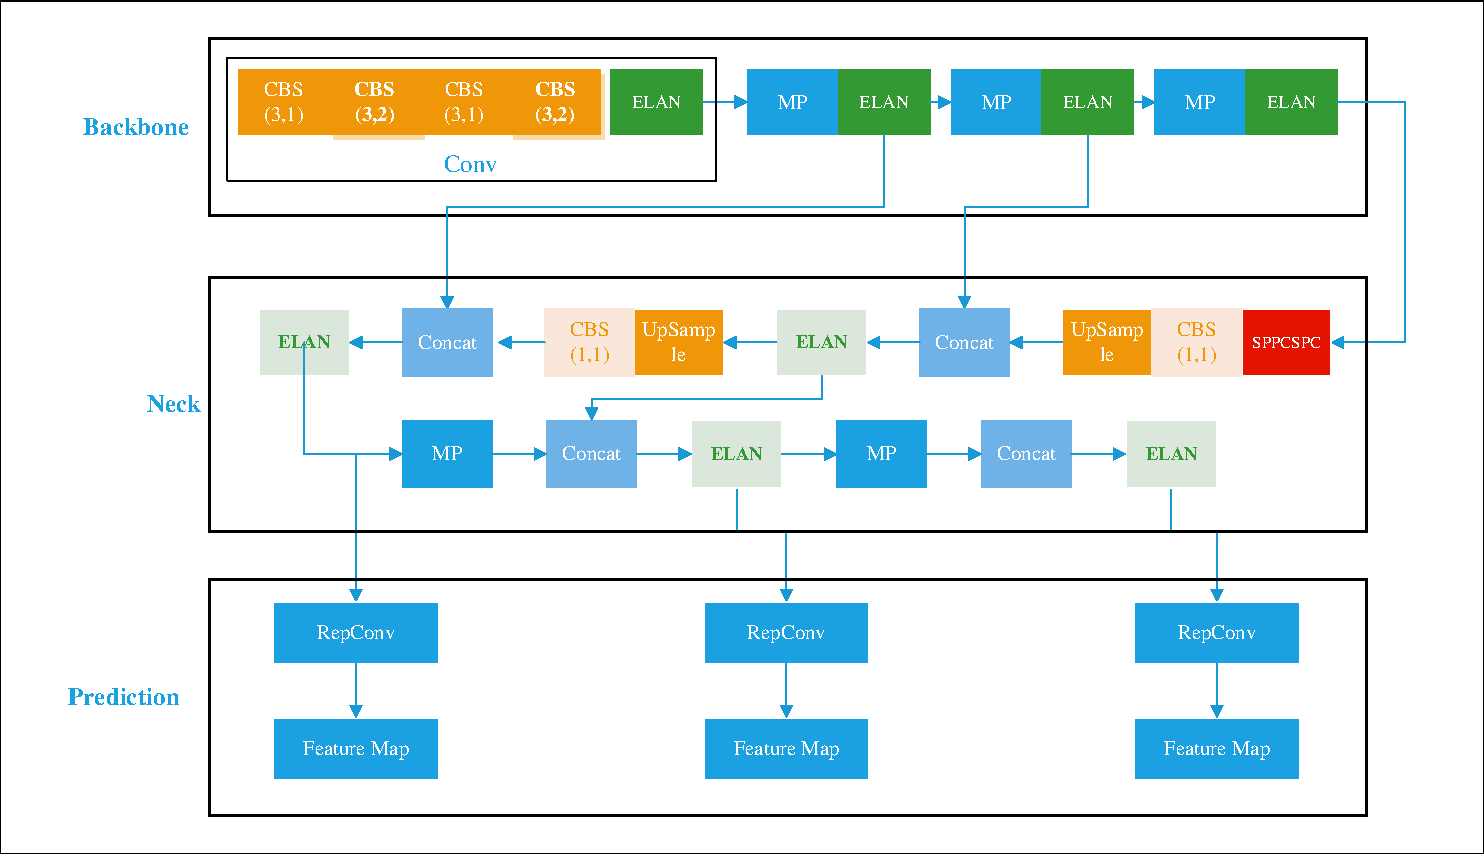
\includegraphics[width=0.45\textwidth]{yolov7_structure.pdf}
    \caption{The architecture of YOLOv7}
    \label{fig:Structure_of_YOLOv7}
\end{figure}

The YOLOv7 algorithm is widely applied in diverse object detection scenarios, and its network model is predominantly composed of Input, Backbone, Neck, and Head components, as shown in Figure \ref{fig:Structure_of_YOLOv7}. More specifically, the input layer consists of preprocessed and normalized image inputs, and the backbone network is responsible for extracting features from input images. The Head layer in YOLOv7 is a CSPSPP layer, so it is merged into the Neck layer in the image. 

The multi-layer ELAN (Efficient Layer Aggregation Networks) structure is designed to enhance computational efficiency and strengthen feature fusion capabilities. This structure employs complex layer aggregation strategies to significantly improve feature extraction performance, making it more suitable for object detection tasks. Specifically, the ELAN architecture consists of basic units made up of multiple convolutional layers, activation functions (such as ReLU or Leaky ReLU), and normalization layers (such as Batch Normalization), which are further combined into higher-level groups. ELAN achieves parallel feature processing by aggregating outputs from multiple convolution paths at specific nodes, thereby enriching feature expression diversity. At the same time, ELAN emphasizes multi-scale feature aggregation, integrating information from different layers through feature fusion, and it alleviates the vanishing gradient problem with skip connections similar to those in ResNet, thus enhancing training stability and efficiency.

However, the original multi-layer ELAN structure in YOLOv7 results in substantial inter-layer information exchange, thereby decelerating the algorithm's training speed. Additionally, the utilization of fixed anchor sizes in YOLOv7 confines its effectiveness in discerning and detecting objects with various scales, particularly in demanding scenarios. These demanding scenarios can include conditions such as poor lighting, occlusion, or objects in high-speed motion, which complicate the detection process.

In object detection, another major challenge is the limitation of the YOLO algorithm in detecting small targets, especially in complex traffic environments. Due to the small size of these targets and their low pixel resolution, they often contain limited information in the image, making them susceptible to interference or occlusion from the background.

It is widely recognized that increasing the number of parameters and utilizing more intricate networks can partially enhance the accuracy of algorithmic detection. However, concerning detection accuracy, the effectiveness of improving training time and model size is restricted. Moreover, in engineering applications, the use of complex networks and a high volume of parameters is non-ideal owing to the computational constraints at the application level. Therefore, the presented algorithm strives to enhance the efficiency of the network layers instead of further augmenting the complexity of the YOLOv7 base model.

To tackle the challenges of detecting small targets in complex scenes, this paper proposes an improved YOLOv7 object detection algorithm based on the YOLOv7 network. The algorithm enhances the accuracy of target localization and recognition while retaining the fundamental features of the YOLOv7 network. This model differs from existing methods in that it does not require multi-scale feature fusion. Instead, it introduces the SimAM attention mechanism, which enables the network to learn and emphasize important aspects of the targets without introducing additional parameters. Additionally, the algorithm improves efficiency while maintaining detection accuracy by redesigning the original backbone network. By replacing the loss function used in the YOLOv7 algorithm, its recognition capability is enhanced, improving both parallelism and stability. Experimental results demonstrate that the improved YOLOv7 algorithm performs exceptionally well in handling complex scenes and small targets, effectively overcoming the aforementioned challenges.

\section{SAM-YOLO algorithm} \label{sec:improved_algorithm}

SAM-YOLO is an improved target detector based on the YOLOv7 architecture. The algorithm focuses on the challenges of small target detection in complex scenarios and improves the accuracy of target localization and identification while retaining the basic features of the YOLOv7 network while minimizing the potential degradation of target detection accuracy and recall. In addition, SAM-YOLO effectively reduces the number of parameters required for the model and speeds up the inference of the model. The network structure is shown in Fig. \ref{fig:improved_YOLOv7}, and the main improvements are as follows:

\begin{enumerate}
    \item Incorporating the SimAM mechanism into the backbone network by designing experiments
    \item Redesigning the backbone network of the model
    \item Replacing part of the original structure with the more lightweight C3 module
    \item Redesigning the loss function of the model
\end{enumerate}

\subsection{SimAM attention mechanism}

The attention mechanism is a widely used technique in the fields of machine learning and deep learning. It aims to simulate the human attention mechanism, selectively focusing on important parts of the input data. The attention mechanism has been extensively studied and applied in various tasks, including natural language processing, computer vision, and speech recognition. By introducing the attention mechanism, models can pay more attention to the parts that are more important for the current task when processing large amounts of information. The core idea of this mechanism is to determine the importance of each element in the input data through learning weight allocation. In the attention mechanism, each element can be assigned a weight or attention score, which reflects the model's degree of attention to each element. The model can adaptively adjust these weights based on the characteristics of different tasks and input data, thereby making more accurate predictions and processing.

The application of attention mechanisms in the fields of machine learning and deep learning is very extensive, including several important attention mechanisms such as CBAM, CA, SE, and SimAM. \cite{cheng2024enhancing,shen2023ca-yolo,jia2023mobilenet-ca-yolo,wu2023yolo-se,mahaadevan2023automatic}


CBAM (Convolutional Block Attention Module) is an attention mechanism based on convolutional neural networks. It enhances model performance by capturing both channel attention and spatial attention. Channel attention is used to determine the importance of each channel in the input feature map, thereby weighting the channels. Spatial attention, on the other hand, determines the importance of each spatial position in the feature map, thus weighting the elements at different spatial positions. By combining channel attention and spatial attention, the CBAM attention mechanism enables the model to more accurately focus on the important parts of the input data.

The CA (Channel Attention) mechanism focuses on channel attention to determine the importance of each channel in the feature map. By utilizing global average pooling and fully connected layers, the CA attention model can compute and allocate weights for each channel to better capture the feature representations of different channels. The CA attention mechanism performs well in computationally intensive tasks and helps the model differentiate the importance of each channel more effectively.

The SE (Squeeze-and-Excitation) attention mechanism is a lightweight attention model that enhances the representation capability of the model efficiently. The core idea of the SE attention model is to dynamically adjust the weights of each channel by utilizing global contextual information. By introducing the "squeeze" and "excitation" stages, the SE attention mechanism can adaptively learn the importance of each channel and re-weight the features accordingly. The SE attention mechanism has achieved good results in many image classification and object detection tasks.

\citeauthor{Yang2021} propose a module that efficiently generates true 3D weights in SimAM \cite{Yang2021}. Specifically, it estimates the importance of individual neurons by taking into account the phenomenon in neurology where over-excited neurons usually inhibit surrounding neurons. This phenomenon suggests that neurons with spatial inhibition effects should be assigned higher weights in visual processing. The importance of each neuron is determined based on its linear separation from other neurons using the formula defined as Equation \ref{eq:energy_function}.

\begin{equation}
 e_t^* = \frac{4 ( \hat{\sigma} ^ 2 + \lambda )}{(t - \hat{\mu}) ^ 2 + 2 \hat{\sigma} ^ 2 + 2 \lambda}  \label{eq:energy_function}
\end{equation}

Theoretically, $\hat{\mu}$ represents the average of individual neurons, and $\hat{\sigma}$ denotes the variance of individual neurons. Equation \ref{eq:energy_function} demonstrates that a lower neuron energy $e^t$ indicates a greater dissimilarity between the neuron and its neighboring neurons, resulting in a correspondingly higher weight. $\lambda$ is a hyperparameter introduced to stabilize the attention map during its computation. It represents a small positive value added to prevent division by zero and to improve numerical stability in the calculation of the attention weights. If $\lambda$ is too small, the division by nearly zero might lead to extremely high attention values, which might dominate the learning process and lead to poor generalization. Conversely, if it's too large, it may overly smooth out the differences in attention, leading to underfitting. In our cases, $1e^{-4}$ was used in our experiment.  Consequently, the significance of a neuron can be determined using $\frac{1}{e_t^{*}}$. Moreover, the algorithm reintroduces the concept of neurology and proposes that attention regulation in the mammalian brain commonly involves the amplification or scaling of neuronal responses, instead of mere addition or subtraction. Thus, the algorithm applies a scaling operation to the neuronal energy $e^t$ to amplify its characteristics. Here, $E$ represents the sequence of energy $e^t$ of all neurons in both channel and space.

Computationally, $\hat{\mu}$ represents the average value of all neurons within a channel over the spatial dimensions (i.e., height $H$ and width $W$). 

\begin{equation}
    \hat{\mu} = \frac{1}{H \times W} \sum_{i=1}^{H} \sum_{j=1}^{W} X_{:, :, i, j}
\end{equation}
where $X_{:, :, i, j}$ represents all neurons at position $(i, j)$ within the channel.

Variance $\hat{\sigma}^2$ describes the degree of dispersion of neurons around the calculated spatial mean. It is computed using the formula: 

\begin{equation}
\hat{\sigma}^2 = \frac{1}{H \times W - 1} \sum_{i=1}^{H} \sum_{j=1}^{W} (X_{:, :, i, j} - \hat{\mu})^2
\end{equation} 

Here, "-1" is used to provide an unbiased estimate.

Neuron energy $e^t$ reflects the similarity of a neuron to its neighboring neurons. Lower energy indicates a greater difference between the neuron and its neighbors, thus possibly being more significant. 

\begin{equation}
    \tilde{X} = \frac{1}{e_t^{*}} \label{eq:energy_sigmod}
\end{equation}

The importance of each neuron is determined by the linear separability defined in Equation \ref{eq:energy_sigmod}, and the sigmoid function is employed to prevent the reciprocal of $E$ from becoming excessively large. Moreover, as the $sigmoid$ function is monotonically increasing, it preserves the relative weights between neurons.

\begin{table*}[!htbp]
    \caption{Test Result On Different Attention Mechanism}
    \label{tab:SimAM_effect}
    \centering
    \begin{tabular}{cccccc}
        \toprule
 Mechanism & Params(\%) & Precision \% & Recall \% & $mAP_{0.5}$ & $mAP_{0.5:0.95} $ \\ \midrule       
 SimAM     & +0\%       & 0.958        & 0.889     & 0.895       & 0.684             \\      
 CBAM      & +0.5\%     & 0.957        & 0.859     & 0.905       & 0.700             \\       
 CA        & +0.2\%     & 0.961        & 0.852     & 0.905       & 0.695             \\      
 SEAM      & +0.9\%     & 0.905        & 0.830     & 0.883       & 0.608             \\\bottomrule    
    \end{tabular}
\end{table*}

To determine the impact of the SimAM module on different parts of YOLOv7, we conducted a series of experiments to evaluate the architecture of the SimAM module that has the greatest positive impact on evaluation indicators. Specifically, we integrated the SimAM module into the input network, backbone network, neck network, and head network of YOLOv7 by replacing certain layers within the original architecture.  We then compared the model performance before and after the SimAM module's integration. The experimental results show that the SimAM module has the greatest impact on the neck network of YOLOv7. After introducing the SimAM module, the performance of the backbone network of YOLOv7 has significantly improved. Table \ref{tab:SimAM_effect} shows detailed experimental results on our collected datasets.

\begin{table*}[!htbp]
    \centering
    \caption{The Impact of SimAM Module on YOLOv7}
    
    \begin{tabular}{ccccc}
        \toprule
 Location            & Precision \% & Recall \% & $mAP_{0.5}$ & $mAP_{0.5:0.95}$ \\ \midrule
 Backbone (Layer 12) & 0.890        & 0.773     & 0.844       & 0.556            \\
 Neck (Layer 64)     & 0.928        & 0.820     & 0.886       & 0.607            \\
 Neck (Layer 76)     & 0.958        & 0.889     & 0.895       & 0.684            \\
 Neck (Layer 102)    & 0.922        & 0.863     & 0.895       & 0.642            \\ \bottomrule
    \end{tabular}
\end{table*}

In the SAM-YOLO model, the SimAM attention mechanism substitutes a segment of the ELAN structure within the Neck layer. More precisely, the SimAM module replaces the initial six convolutional layers, featuring {1, 1} as the step size parameter and {3, 1} as the convolution kernel size parameter. During forward propagation, SimAM evaluates the neurons and activates them based on Equation \ref{eq:energy_sigmod}.

\subsection{Loss function}

In machine learning, the loss function serves as a metric for evaluating the discrepancy between the predicted and actual values of a model. By continuously adjusting its parameters to minimize this discrepancy, the model's performance can be improved, leading to better detection and prediction accuracy.

Meanwhile, during object detection, the algorithm generates multiple bounding boxes with high confidence around the target object. However, only one bounding box can accurately represent the target. To address this redundancy, a non-maximum suppression (NMS) algorithm is implemented, which ensures that only the most appropriate bounding box is selected. The algorithm starts by sorting all bounding boxes and then calculates the Intersection over Union (IoU) of the highest-confidence bounding box with the remaining boxes. If the IoU of a bounding box exceeds a predefined threshold, it is discarded.

To evaluate the performance of image segmentation models, the Intersection over Union (IoU) metric is commonly employed. This metric quantifies the degree of overlap between predicted and ground truth boxes, thereby assessing the accuracy of predictions made by the model.

\begin{equation}
 IoU = \frac{\left\lvert B \cap B^{gt} \right\rvert }{\left\lvert B \cup B^{gt} \right\rvert } \label{eq:IoU}
\end{equation}

The formula for calculating IoU, as presented in Equation \ref{eq:IoU}, typically utilizes the norm of IoU. In this equation, $B$ represents the ground truth box with four parameters: $x$, $y$, $w$, and $h$, which respectively indicate the coordinates of the box center, as well as the width and height of the box. $B^{gt}$ denotes the predicted box. The IoU-based loss function $\mathfrak{L}$ is defined in Equation \ref{eq:IoU_loss}. A smaller value of $\mathfrak{L}$ indicates a more effective detection outcome from the model.

\begin{equation}
    \mathfrak{L}_{IoU}= 1 - \frac{\left\lvert B \cap B^{gt} \right\rvert }{\left\lvert B \cup B^{gt} \right\rvert }  \label{eq:IoU_loss}
\end{equation}

\begin{equation}
    \mathfrak{L}_{SIoU} = 1 - IoU+ \frac{\Delta + \Omega}{2} \label{eq:SIoU_loss}
\end{equation}

Building upon this foundation, the $CIoU$ loss function used in YOLOv7 is replaced with the $SIoU$ loss function proposed by Gevorgyan and Zhora \cite{Gevorgyan-225}. This loss function comprehensively considers four aspects: angle, distance, shape, and IoU. The resulting loss function, represented in Equation \ref{eq:SIoU_loss}, takes into account the contribution of $\Delta$ (the distance between the center points of the two boxes) and $\Omega$ (the difference in area between the two boxes), in addition to IoU. The schematic diagram of the $SIoU$ loss function is illustrated in Figure \ref{fig:SIoU_loss}.

\begin{figure}[htbp]
    \centering
    \resizebox{0.4\textwidth}{!}{
        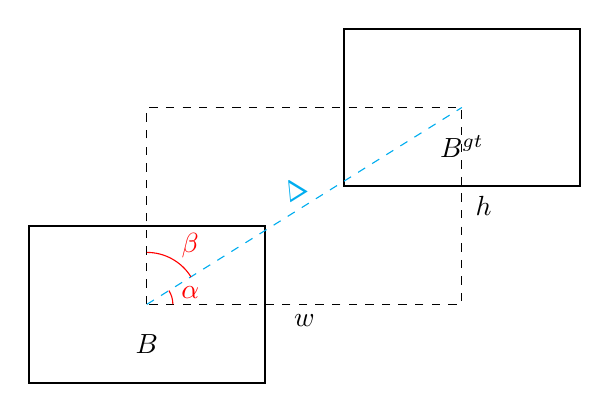
\begin{tikzpicture}
            \def\bx{3}
            \def\by{2}
            \def\dx{4}
            \def\dy{2.5}
            \draw[thick] (0 - \bx / 2, 0 - \by / 2) rectangle (0 + \bx / 2, 0 + \by / 2) ;
            \node at (0, 0 - 0.5) {$B$};
            
            \draw[thick] (\dx - \bx / 2, \dy - \by / 2) rectangle (\dx + \bx / 2, \dy + \by / 2);
            \node at (\dx, \dy - 0.5) {$B^{gt}$};
            % third rectangle center at (\dx / 2, \dy / 2)
            \draw[dashed] (0, 0) rectangle (\dx, \dy);
            \draw[dashed, cyan] (0, 0) -- (\dx, \dy) node[midway, above, sloped] {$\Delta$};
            \node[below] at (\dx / 2, 0) {$w$};
            \node[left] at (\dx + 0.5, \dy / 2) {$h$};
            \pgfmathsetmacro{\anglerec}{atan(\dy / \dx)}
            
            \draw[red, -] (0.33, 0) arc (0:\anglerec:0.33);
            \draw[red, -] (0, 0.66) arc (90:\anglerec:0.66);
            \node[red] at (0.55, 0.15) {$\alpha$};
            \node[red] at (0.55, 0.75) {$\beta$};
            
        \end{tikzpicture}
        
 }
    
    \caption{The schematic diagram of $SIoU$ loss function}
    \label{fig:SIoU_loss}
\end{figure}

Where $\Delta$ represents the distance between the center points of two boxes, $\Omega$ represents the difference in area between the two boxes, and $IoU$ represents their intersection. A smaller value of $\mathfrak{L}$ indicates a better detection effect of the model.

The $SIoU$ loss function assigns different weights to object detection at various scales, giving more attention to objects with smaller scales during training. By introducing additional variables, such as shape loss, the $SIoU$ function not only provides a better measure of symmetry between the predicted box and the true box but also addresses the imbalance problem found in other $IoU$ variants. Additionally, it facilitates faster convergence to the optimal solution and reduces training time. Moreover, it possesses greater sensitivity in detecting small target objects, thereby reflecting the effectiveness of the target detection model more accurately.

\subsection{Construction network of the SAM-YOLO}

In the SAM-YOLO algorithm, YOLOv7 is adopted as the basic network architecture, and the C3 module is incorporated. The number of layers and parameters in the network is reduced through this module, accelerating the model's inference and training speed.

Furthermore, the SimAM attention mechanism is introduced into the Neck network. This parameterless attention algorithm proposes an energy function based on mathematical methods to determine the importance of each neuron. Inspired by concepts in neurology, this approach avoids expending excessive energy on adjusting and enhancing the structure. Figure \ref{fig:improved_YOLOv7} illustrates the improved architecture of the algorithm.

\begin{figure*}[htbp]
    \centering

    \begin{tikzpicture}
        % 包含图像
        \node[anchor=south west,inner sep=0] (image) at (0,0) {
            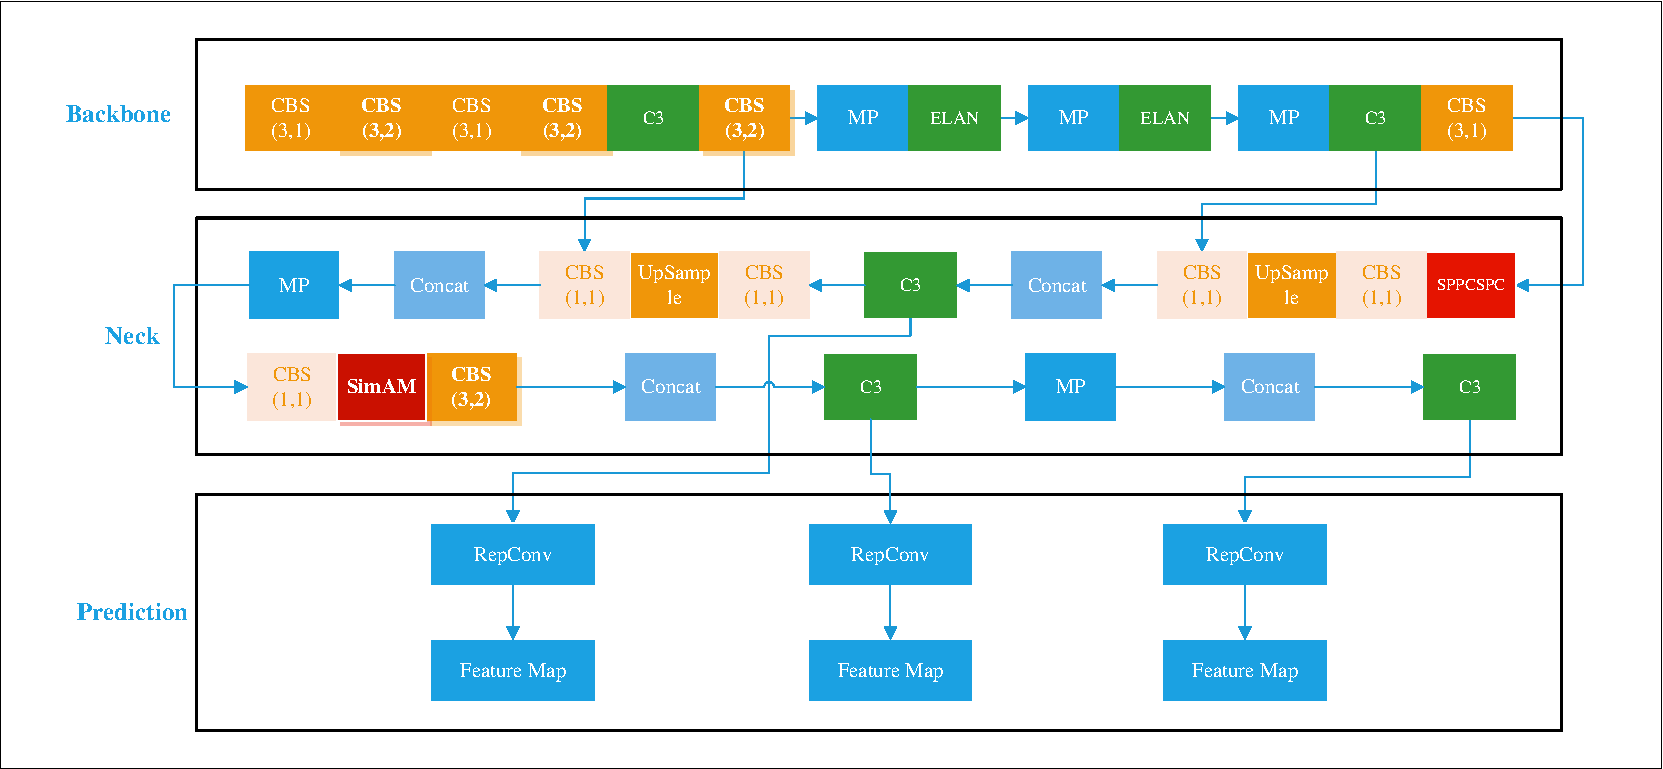
\includegraphics[width=\textwidth]{improved_structure.pdf}
 };

        % 获取图像边界
        \begin{scope}[x={(image.south east)},y={(image.north west)}]
            % 添加半透明矩形遮罩,(0.2,0.3) 是左下角坐标,(0.6,0.7) 是宽度和高度
            \draw[red,thick] (0.14,0.42) rectangle (0.32,0.55);

            % 添加文本标注
            % \node at (0.4,0.5) [align=center, opacity=0.8] {\textbf{aaa}};
        \end{scope}
    \end{tikzpicture}
    \caption{The architecture of the improved algorithm}
    \label{fig:improved_YOLOv7}
\end{figure*}

\section{Experiment and Analysis} \label{sec:experiment_and_analysis}

\subsection{The Dataset}

To ensure the applicability of the vehicle recognition model on highways and urban roads, we collected a substantial number of authentic road videos captured by vehicle dashcams or built-in cameras near Xiangyang City, China, on highways and urban roads. The videos were captured from the driver's front-facing perspective encompassing diverse road and driving scenarios, including clear weather conditions on two-way four-lane roads, dimly lit rural road scenes, capturing traffic signs, vehicles, pedestrians, traffic lights, and road markings while vehicles are in motion. Figure \ref{fig:clear_condition}, \ref{fig:cloudy_condition}, \ref{fig:night_condition} displays images from the training set, capturing different types of vehicles from various angles, road segments, and lighting conditions to enhance the dataset diversity. Figure \ref{fig:clear_condition} displays images captured in clear weather conditions, Figure \ref{fig:cloudy_condition} displays images captured in cloudy weather conditions, and Figure \ref{fig:night_condition} displays images captured at night or in tunnels.

\begin{figure}[htbp]
    
    \centering    
    \subfigure[Clear weather condition]{
        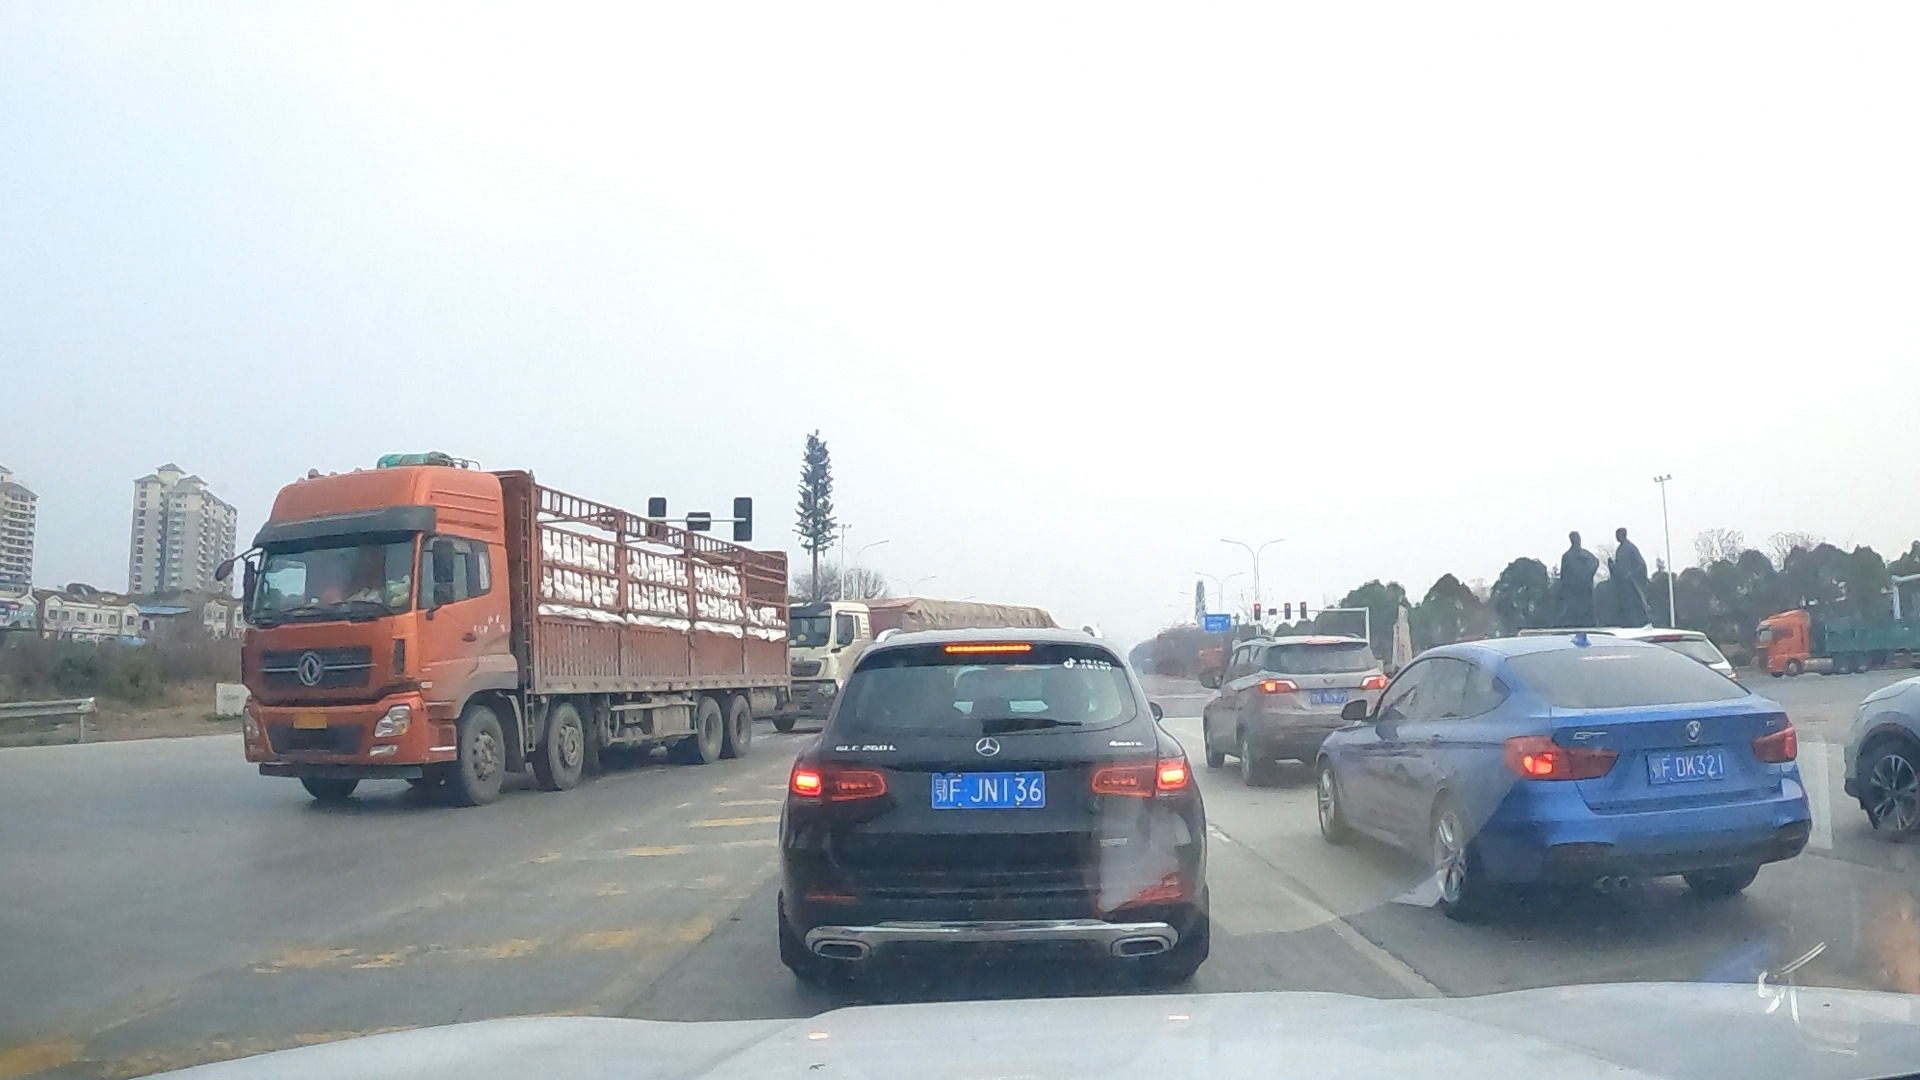
\includegraphics[width=0.2\textwidth]{clear (2).jpg}
        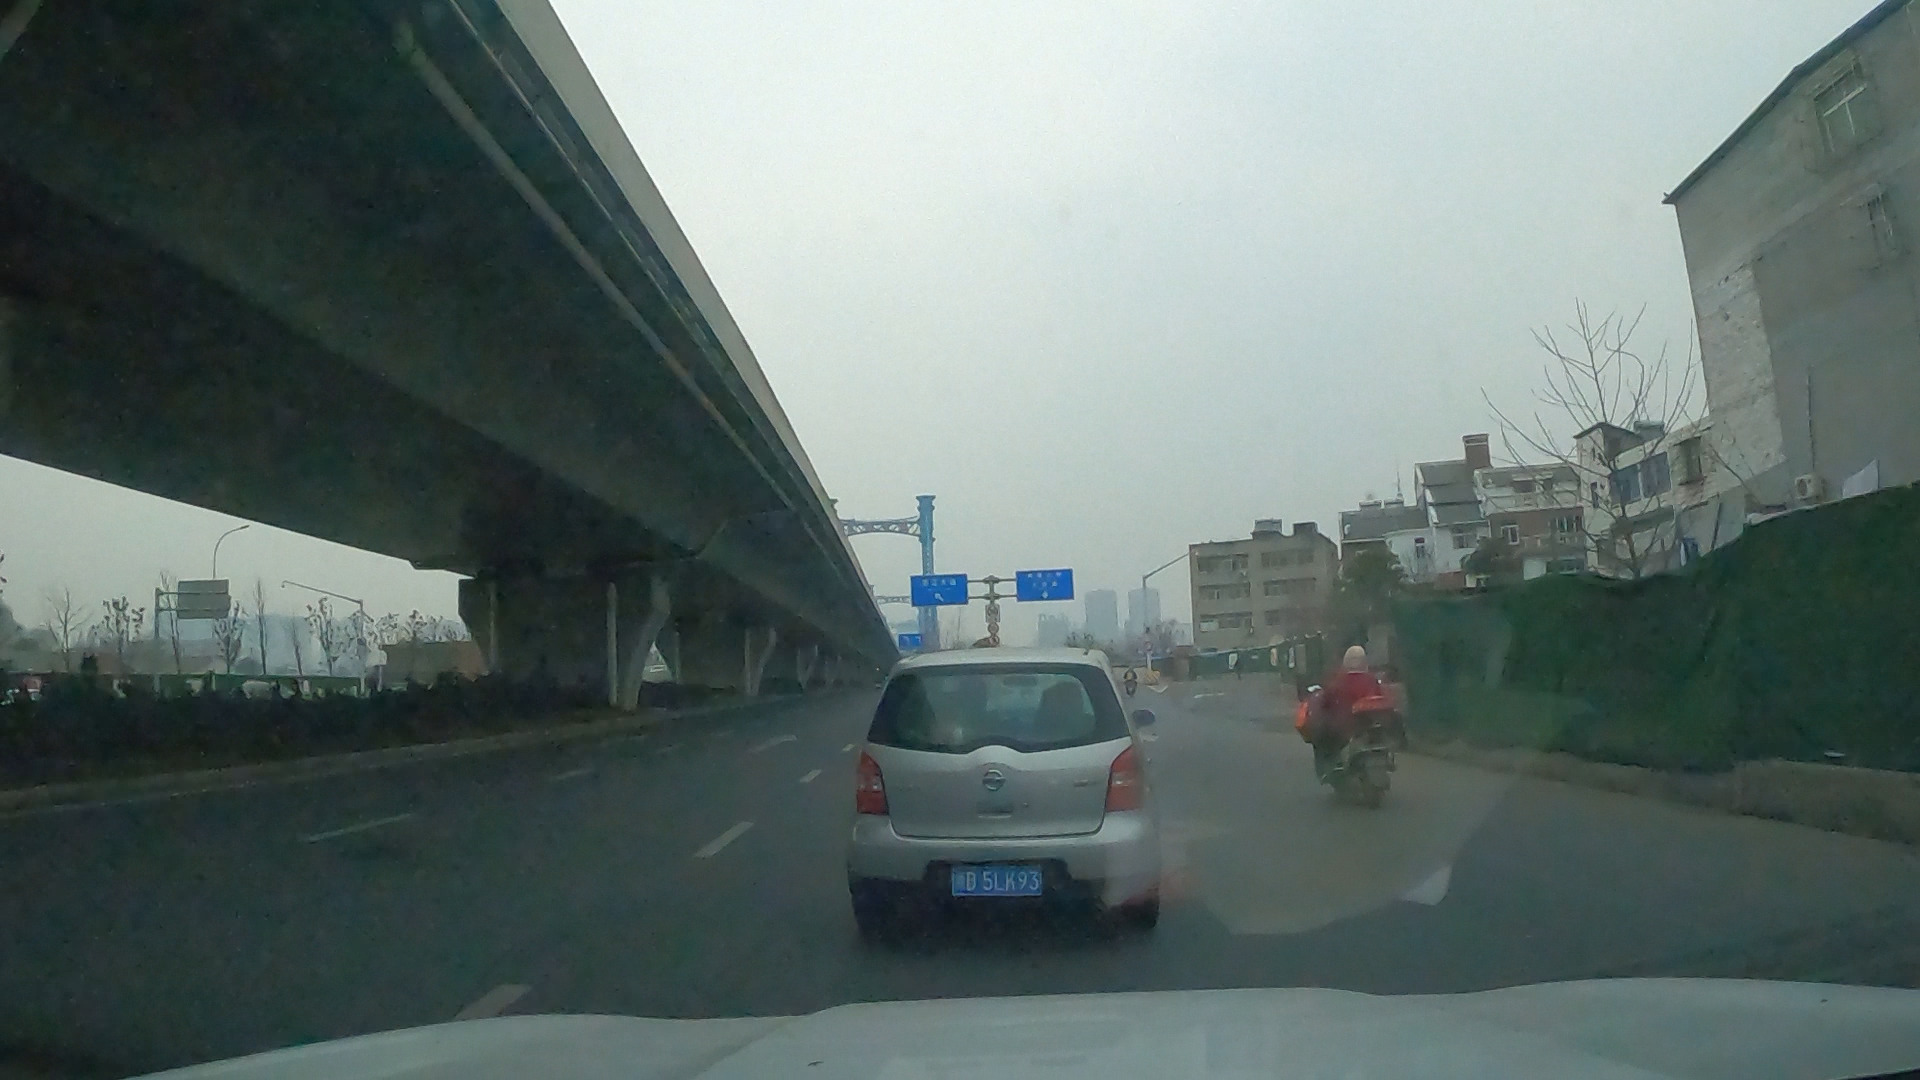
\includegraphics[width=0.2\textwidth]{clear (1).jpg}
        \label{fig:clear_condition}
        
 }
    
    \subfigure[Cloudy weather condition]{
        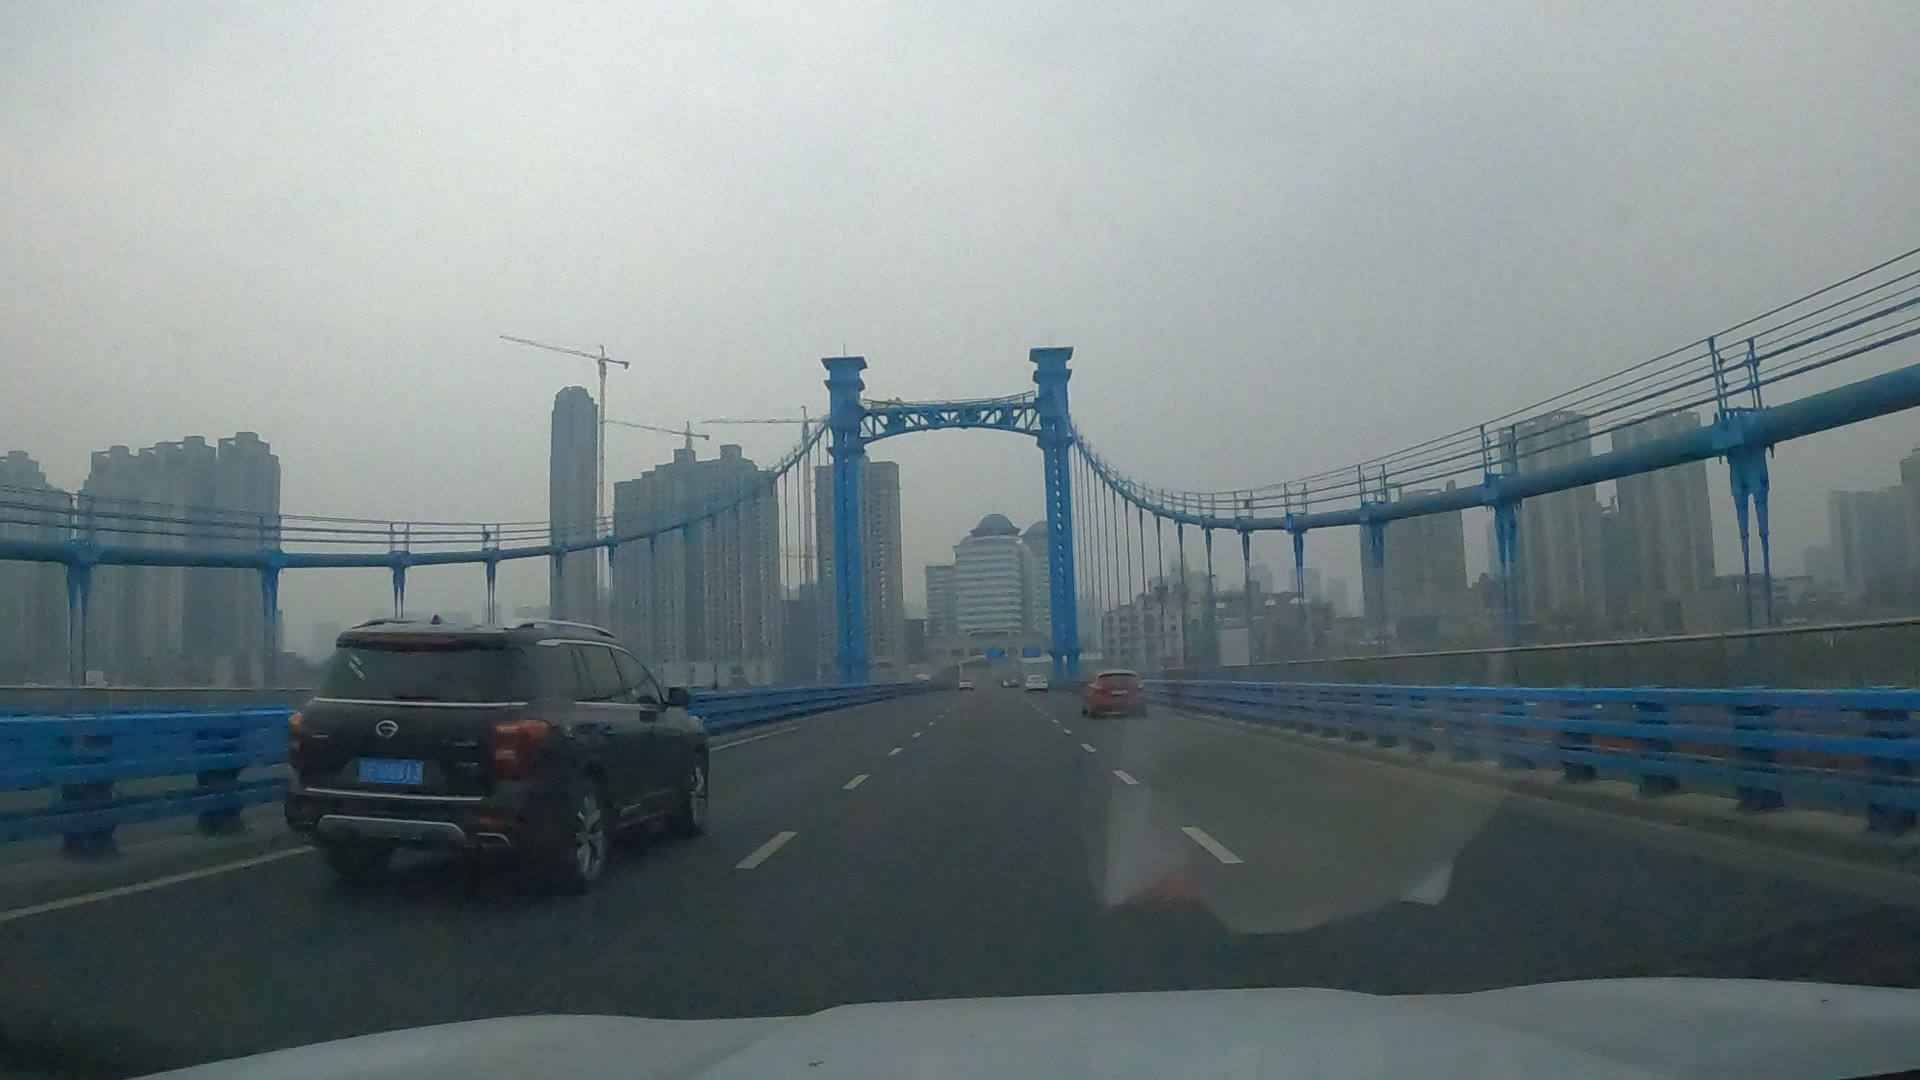
\includegraphics[width=0.2\textwidth]{cloudy (1).jpg}
        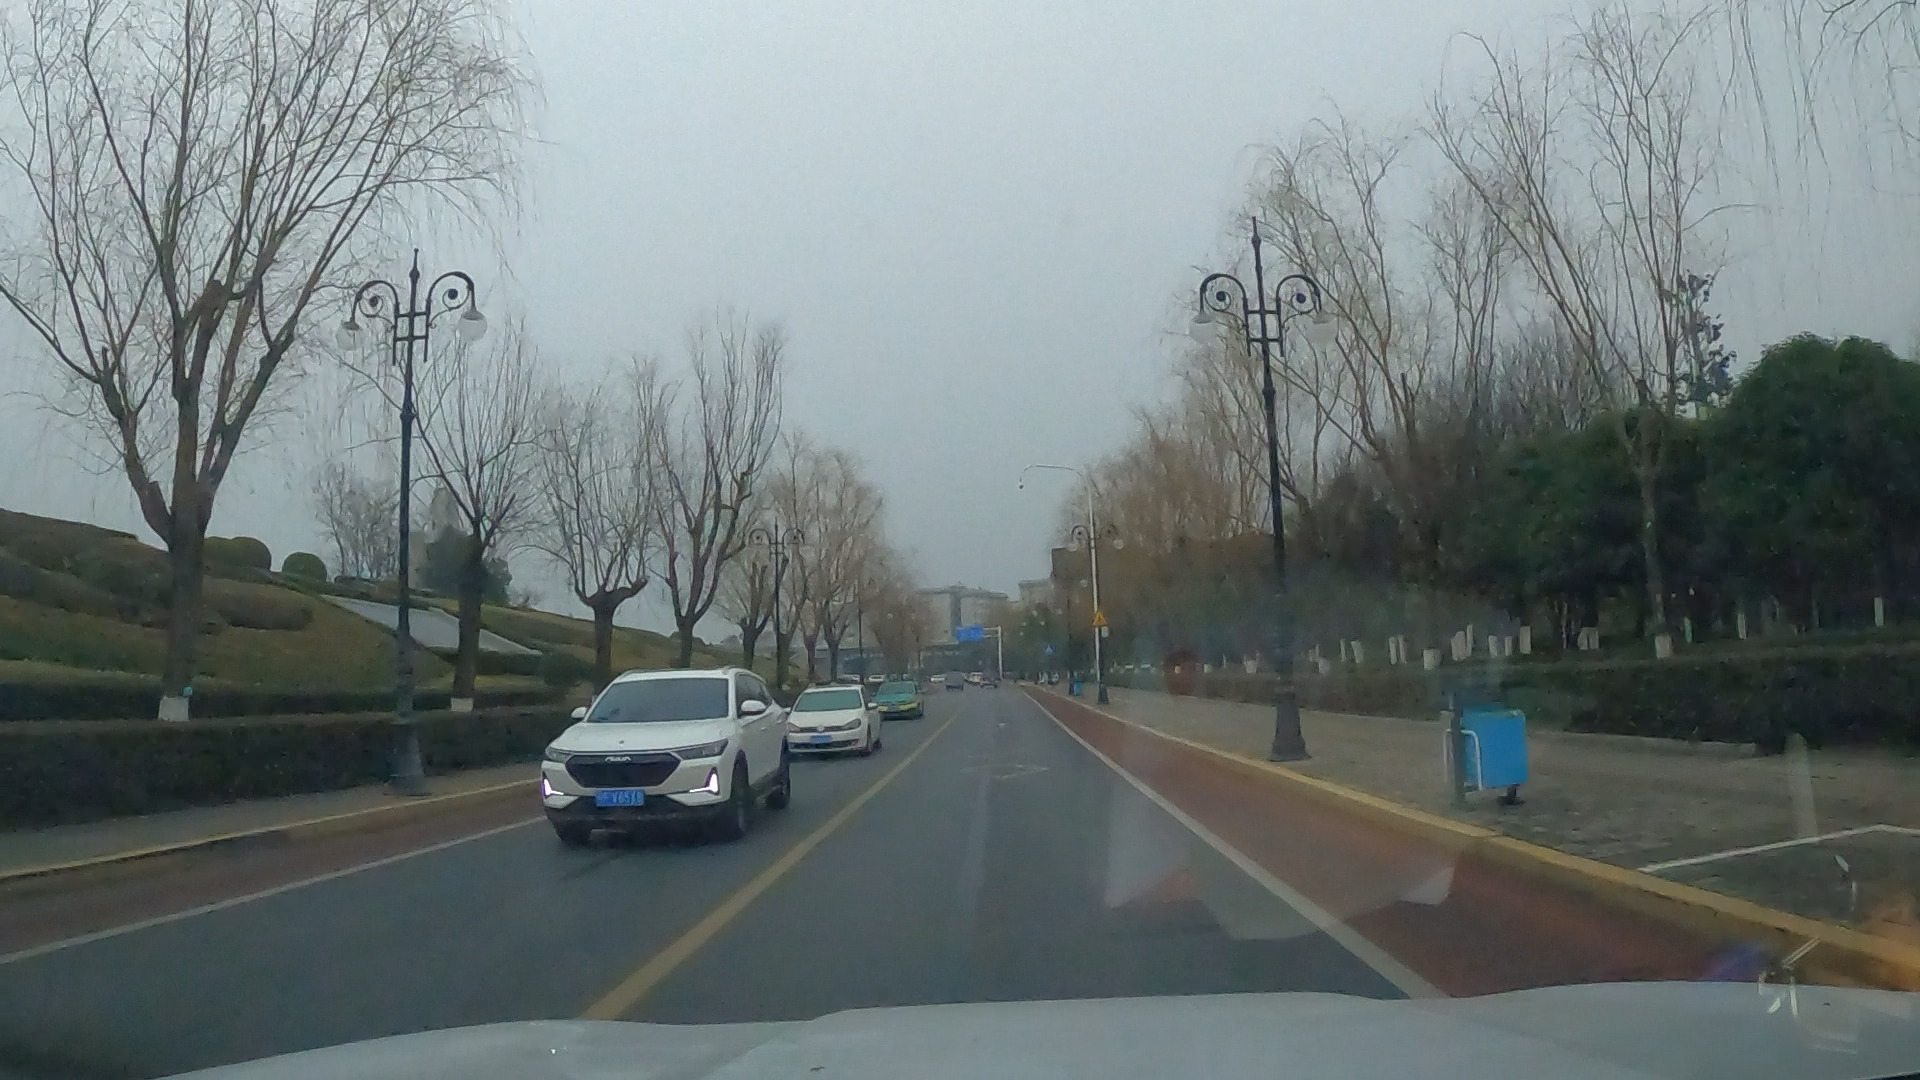
\includegraphics[width=0.2\textwidth]{cloudy (2).jpg}
        \label{fig:cloudy_condition}
 }
    
    \subfigure[Night or tunnel condition]{
    
        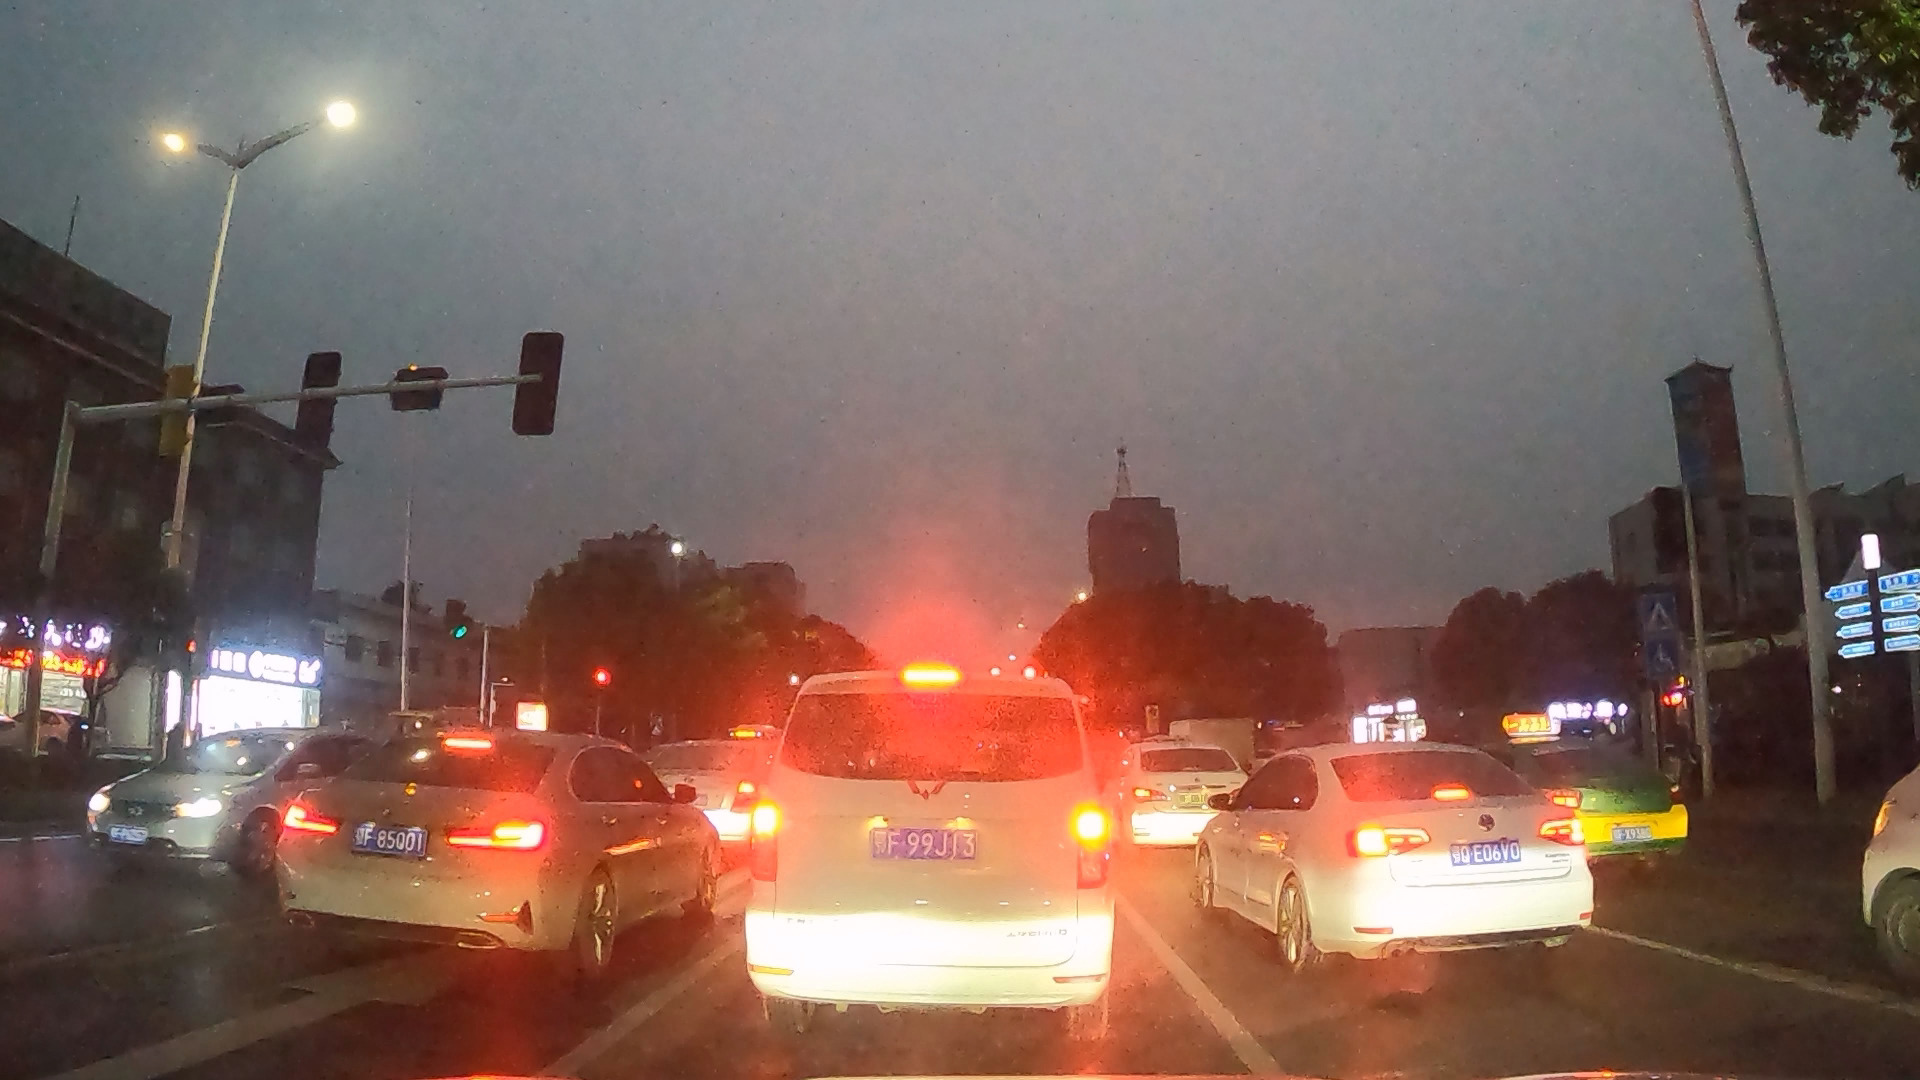
\includegraphics[width=0.2\textwidth]{night (2).jpg}
        
        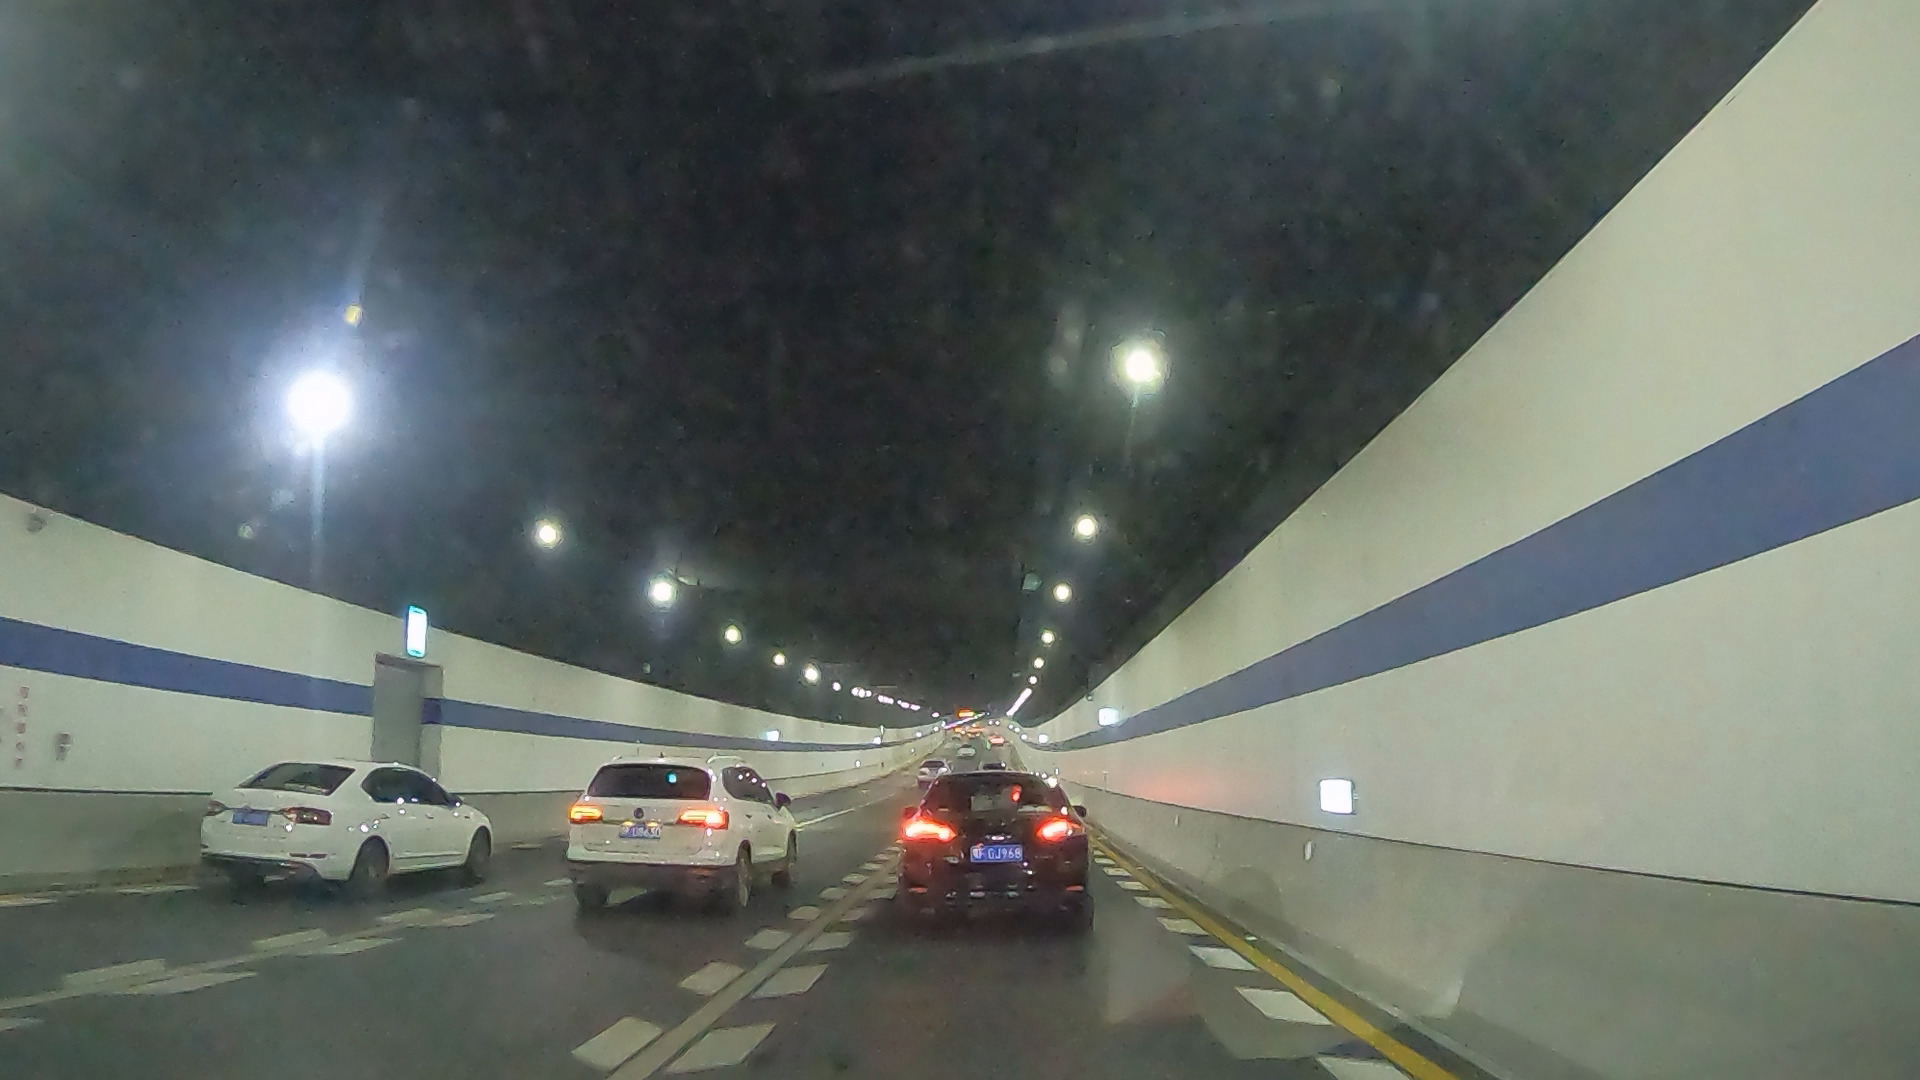
\includegraphics[width=0.2\textwidth]{night (1).jpg}
        
        \label{fig:night_condition}
        
 }
    \caption{Images from the training set}

    
\end{figure}

Segments with a high number of vehicles and clear video quality were meticulously selected, and one image sample was extracted for every 25 frames. Ultimately, a dataset of 16,008 images with vehicle information was obtained, encompassing various vehicle categories such as cars, trucks, taxis, and tankers. To ensure proper evaluation, the dataset was divided into training, validation, and test sets in a ratio of $7:2:1$. The training set comprises 11,206 frames, the validation set comprises 3,198 frames, and the test set comprises 1,604 frames.

\subsection{Data Augmentation}

Videos captured by dashcams or in-vehicle cameras, while partially representative of real road scenarios are influenced by various factors. Challenges such as image blurring from camera focus issues, underexposed or overexposed objects due to high contrast, and video noise from lighting conditions introduce recognition noise to the captured images. These issues hinder the training effectiveness of machine learning models.

To address this, we implement data augmentation during model training to enhance model robustness. Our augmentation techniques include:

\begin{enumerate}
    \item Rotation: Images are randomly rotated between $-10\degree$ and $+10\degree$ to help the model recognize objects regardless of their orientation.
    \item Shear: Horizontal and vertical shearing by $\pm10\degree$ simulates changes in perspective.
    \item Brightness Adjustment: Variation in image illumination by $-30\%$ to $+30\%$ enhances adaptation to fluctuating lighting conditions.
    \item Blur: A blur effect of up to 2 pixels approximates the out-of-focus images.
    \item Noise Addition: Introducing noise to up to $1\%$ of pixels mimics sensor noise or transmission interference.
\end{enumerate}

Additional challenges include motion-induced blur from the movement of objects and the camera's distance, often resulting in out-of-focus images. Gaussian blur, a linear smoothing filter, is utilized to reduce this blur while preserving edge information. The Gaussian kernel is defined as follows:

\begin{equation}
 G(x, y) = \frac{1}{2\pi \sigma^2} \exp \left(-\frac{(x - \frac{N-1}{2})^2 + (y - \frac{N-1}{2})^2}{2\sigma^2} \right)
\end{equation}

Here, $G(x, y)$ denotes the weight at coordinates $(x, y)$ within the 2D Gaussian kernel, which is normalized to ensure the total weight sum is 1.

Additionally, low-light conditions can introduce random image noise, which mere camera adjustments cannot correct. In this context, Poisson noise—a statistical distribution that models random events like photon counting—effectively simulates noise under low light. This approach helps to replicate realistic imaging conditions, further improving the model's robustness.

\subsection{Experimental environment}

The experimental environment utilized in this study is summarized in Table \ref{tab:environment}.

\begin{table}[htbp]
    
    \centering
    
    \caption{Experimental environment}
    
    \label{tab:environment}
    
    \begin{tabular}{cc}
        
        \toprule
        
 Parameters       & Value                     \\
        
        \midrule
        
 Operating system & Ubuntu 23.10              \\
        
 CPU              & Intel Xeon Platinum 8352V \\
        
 GPU              & RTX 4090 (24GB) * 32      \\
        
 RAM              & 1024GB                    \\
        
 CUDA Version     & 12.1                      \\
        
 Python Version   & 3.10.9                    \\
        
 Framework        & Pytorch                   \\
        
 Pytorch Version  & 2.1                       \\
        
        \bottomrule
        
    \end{tabular}
    
\end{table}

% \subsection{Training Parameters}

The training parameters utilized in this experiment are presented in Table \ref{tab:training_parameters}.

\begin{table}[htbp]
    
    \centering
    
    \caption{Training parameters}
    
    \label{tab:training_parameters}
    
    \begin{tabular}{cc}
        
        \toprule
        
 Parameters & Value               \\
        
        \midrule
        
 batch-size & 64                  \\
        
 epochs     & 300                 \\
        
 img-size   & 640                 \\
        
 hyp        & hyp.scratch.p5.yaml \\
        
 weights    & yolov7.pt           \\
        
 workers    & 8                   \\
        
        \bottomrule
        
    \end{tabular}
    
\end{table}

\subsection{Evaluation Metrics}

Performance evaluation of the SAM-YOLO algorithm involves the utilization of multiple metrics to assess the model's quality. For this study, the evaluation metrics employed include Precision Rate (P), Recall Rate (R), mean Average Precision with an IoU recognition threshold of 0.5 ($mAP_{0.5}$), and mean Average Precision within the IoU range of 0.5 to 0.95 ($mAP_{0.5:0.95}$).

Precision represents the probability of correctly predicting a positive sample, whereas recall denotes the probability of accurately identifying a positive sample from the original sample. $mAP_{0.5}$ refers to the mean average precision of the model with an IoU recognition threshold of 0.5, whereas $mAP_{0.5:0.95}$ represents the mean average precision with an IoU range of 0.5 to 0.95. The accuracies $AP_i$ and $mAP$ for each recognition threshold are computed according to Equation \ref{eq:AP}.

In Equation \ref{eq:AP} and Equation \ref{eq:mAP}, which establish the function $p(r)$ to represent the precision and recall rate, where the calculation equations of precision and recall are shown in Equation \ref{eq:precision} and Equation \ref{eq:recall}. $n$ in Equation \ref{eq:mAP} represents the total number of all samples. The area under the $p(r)$ curve in the interval $[0,1]$ represents the $AP$ value.


In Equation \ref{eq:precision} and Equation \ref{eq:recall}, $TP$ represents the number of true positives, $FP$ represents the number of false positives, and $FN$ represents the number of false negatives.

\begin{equation}
 AP = \int_{0}^{1} p(r)dr \label{eq:AP}
\end{equation}

\begin{equation}
 mAP = \frac{1}{n} \sum_{i=1}^{n} AP_i \label{eq:mAP}
\end{equation}

\begin{equation}
 Precision = \frac{TP}{TP + FP} \label{eq:precision}
\end{equation}

\begin{equation}
 Recall = \frac{TP}{TP + FN} \label{eq:recall}
\end{equation}

\subsection{Experimental results}

The effectiveness of the proposed method was evaluated through extensive experiments conducted on a benchmark dataset in this study. The experimental results indicate that the proposed SAM-YOLO algorithm achieves higher accuracy and recall rates compared to the original YOLOv7 algorithm. Additionally, there is a 3\% improvement in the accuracy of $mAP_{0.5}$ and $mAP_{0.5:0.95}$.
\begin{table*}[!ht]
    \caption{Comparison of evaluation indicators results}
    \label{tab:evaluation_indicators}
    \centering
    \resizebox{\textwidth}{!}{
        \begin{tabular}{@{}ccccccccc@{}}
            
            \toprule
            
 Model category    & Precision (\%) & Recall (\%)    & $mAP_{0.5}$ (\%) & $mAP_{0.5:0.95}$ (\%) & GFLOPS & Parameters (Millions) & Time (ms)  & FPS(/s)  \\
            
            \midrule
            
            % YOLOv5            & 95.15          & 86.02          & 92.26            & 71.86                 & \textbf{49.0} & 21.2                  & 15.9         \\
            
 YOLOv7            & 96.45          & 92.15          & 95.06            & 75.44                 & 105.5  & 35.5                  & 12.6        & 79.36 \\   
            \textbf{SAM-YOLO} & \textbf{96.34} & \textbf{93.46} & \textbf{95.96}   & \textbf{75.72}        & 103.3  & \textbf{36.5}         & \textbf{9.5} & 105.\\ 
            \bottomrule
        \end{tabular}
 }
\end{table*}

\begin{table*}[!htbp]
    
    \centering
    
    \caption{Comparison of detection category results}
    
    \label{tab:detection_category}
    
    \resizebox{\textwidth}{!}{
    
        \begin{tabular}{@{}cccccccccccccccccc@{}}
            
            \toprule
            
            \multirow{2}{*}{Model category} & \multicolumn{8}{c}{$mAP_{0.5}$(\%)} &               & \multicolumn{8}{c}{$mAP_{0.5:0.95}$(\%)}                                                                                                                                                                                                                    \\ \cmidrule(lr){2-9} \cmidrule(l){11-18}
            
                                            & Total                               & People        & Bicycle                                  & Tricycle      & Car           & Motorcycle    & Bus           & Truck         &  & Total         & People        & Bicycle       & Tricycle      & Car           & Motorcycle    & Bus           & Truck         \\ \midrule
            
            % YOLOv5                          & 92.4                                & 78.8          & 90.9                                     & 97.5          & 95.8          & 92.8          & 98.7          & 98.2          &  & 73.6          & 48.3          & 63.9          & 80.0          & 83.5          & 65.4          & 83.8          & 83.6          \\
            
 YOLOv7                          & 95.0                                & 86.7          & 91.8                                     & 98.6          & 98.1          & 93.0          & 99.2          & 98.4          &  & 75.5          & 52.0          & 61.4          & 81.1          & 82.9          & 65.7          & 84.5          & 84.8          \\
            
            \textbf{SAM-YOLO}               & \textbf{95.9}                       & \textbf{88.2} & \textbf{94.3}                            & \textbf{99.2} & \textbf{98.3} & \textbf{93.6} & \textbf{99.3} & \textbf{98.3} &  & \textbf{75.5} & \textbf{54.8} & \textbf{65.3} & \textbf{82.0} & \textbf{84.2} & \textbf{66.2} & \textbf{86.3} & \textbf{85.7} \\ \bottomrule
            
        \end{tabular}
        
 }
    
\end{table*}

\begin{figure*}

    \centering
    
    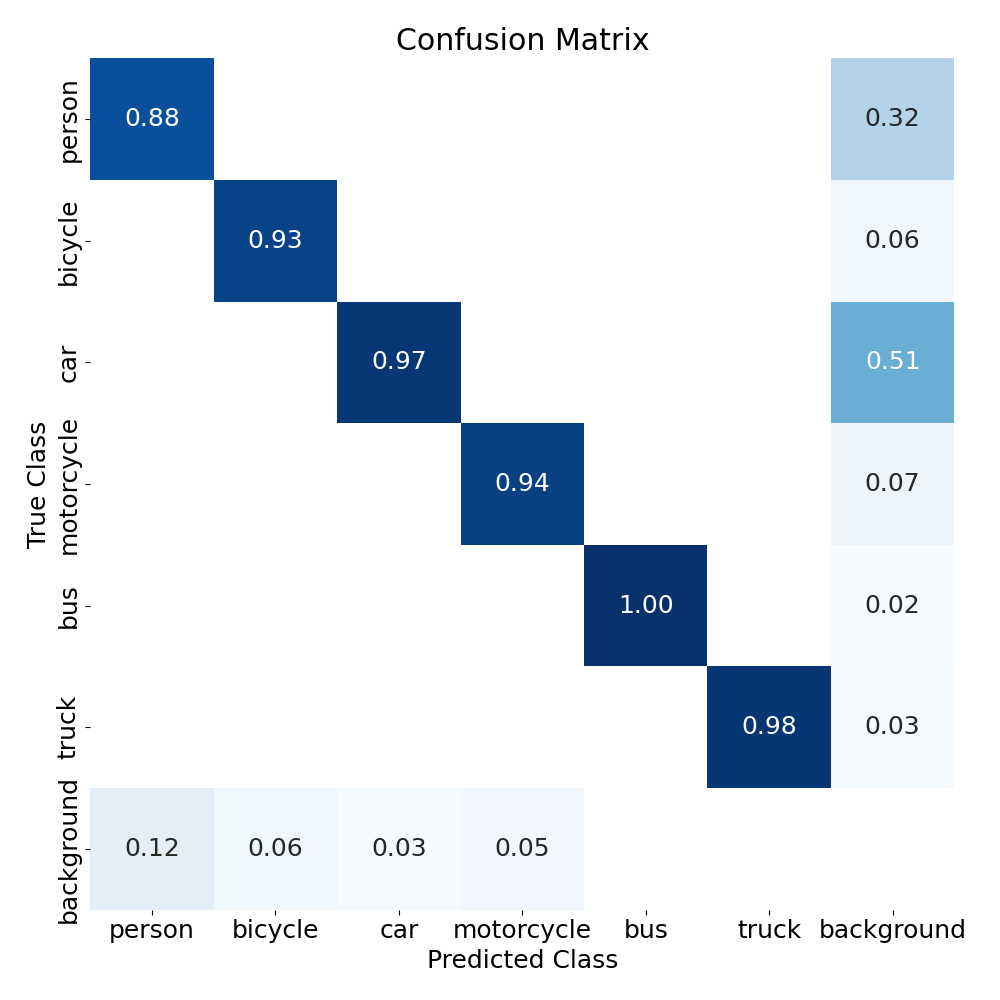
\includegraphics[width=0.6\textwidth]{confusion_matrix.png}
    
    \caption{Confusion matrix of the SAM-YOLO algorithm}
    
    \label{fig:confusion_matrix}
    
\end{figure*}

It can be observed from Figure \ref{fig:confusion_matrix} that the SAM-YOLO algorithm exhibits characteristics of missed detection rate and false detection rate across all detection categories, and demonstrates high accuracy in detecting small targets.

\subsection{Ablation Experiment}

In the ablation experiments conducted, by selectively adding or removing the SimAM, SIoU, and C3 modules, we were able to gain a deeper understanding of the specific impact of these components on the overall performance of the model. The addition or removal of each module provided us with unique insights, which in turn allowed us to meticulously evaluate their respective values and roles. The results of the ablation experiments show that when the SimAM, SIoU, and C3 modules are enabled simultaneously, the model can achieve the highest precision (0.961\%), recall (0.930\%), $mAP_{0.5}$ (0.962), and $mAP_{0.5:0.95}$ (0.725) with a 9.2\% reduction in parameters while maintaining a relatively high frame rate (476 FPS). This suggests that the combined use of these modules can significantly improve the performance of the model.

\begin{table*}[!htbp]
    
    \centering
    
    \caption{Ablation experiment results}
    
    \label{tab:ablation_experiment}
    
    \begin{tabular}{ccccccccc}
        
        \toprule
        
 SimAM      & SIoU       & C3 Module  & Params(\%) & FPS & Precision \% & Recall \% & $ mAP_{0.5}$ & $mAP_{0.5:0.95}$ \\ \midrule
        
        \checkmark &            &            & 0          & 476 & 0.958        & 0.889     & 0.895        & 0.684            \\
        
                   & \checkmark &            & 0          & 312 & 0.946        & 0.853     & 0.908        & 0.649            \\
        
                   &            & \checkmark & -9.2\%     & 312 & 0.944        & 0.860     & 0.913        & 0.658            \\
        
        \checkmark & \checkmark &            & 0          & 434 & 0.933        & 0.847     & 0.925        & 0.623            \\
        
        \checkmark &            & \checkmark & -9.2\%     & 434 & 0.958        & 0.862     & 0.905        & 0.667            \\
        
                   & \checkmark & \checkmark & -9.2\%     & 434 & 0.934        & 0.853     & 0.905        & 0.644            \\
        
        \checkmark & \checkmark & \checkmark & -9.2\%     & 476 & 0.961        & 0.930     & 0.962        & 0.725            \\ \bottomrule
        
    \end{tabular}
    
\end{table*}

\subsection{Comparative Experiment}

In this study, we compare and analyze the performance of multiple target detection algorithms in different contexts, including YOLOv7, SAM-YOLO, CBAM-YOLO, CA-YOLO, SEAM-YOLO, SSD, RetinaNet, and Faster-RCNN.We evaluate the performance of multiple target detection algorithms based on the number of parameters, Frames Per Second (FPS), precision, recall, and different mAP (mean Average Precision) metrics were comprehensively evaluated. All algorithms use ELAN or ResNet-50 as the underlying skeleton to ensure consistency and fairness in the evaluation.

In terms of overall performance, SAM-YOLO performs best in several metrics, especially in $mAP_{0.5}$ and $mAP_{0.5:0.95}$, which reach 0.962 and 0.725, respectively, and are significantly higher than other algorithms. This result indicates that SAM-YOLO is not only able to detect targets efficiently but also has high accuracy and robustness.YOLOv7 also shows strong performance, especially on the FPS metric, which reaches 476, which means that it can realize high-speed real-time target detection.

In the $mAP_{0.5}$ and $mAP_{0.5:0.95}$ evaluations for different object categories, SAM-YOLO has the best performance in almost all categories, especially in "tricycle", "bus" and "tricycle". Especially in the categories of "tricycle", "bus" and "truck", its $mAP_{0.5}$ is as high as 0.993, 0.987, and 0.991, respectively, which is much better than other algorithms. This further confirms the superiority of SAM-YOLO in dealing with complex scenes and targets of different scales.

In contrast, the performance of SSD, RetinaNet, and Faster-RCNN is relatively weak, especially in the $mAP_{0.5:0.95}$ metric, where these algorithms significantly lag behind the improved YOLO-based algorithms. In addition, the large parameter reduction of these algorithms, although conducive to reducing the computational complexity, may also affect the accuracy and comprehensive performance of the detection.

The experimental results show that SAM-YOLO and YOLOv7 are the optimal choices for target detection tasks with high speed and high accuracy. They are not only able to accurately detect various types of targets in complex scenes but also maintain high processing speed to meet the demands of real-time applications. Future research can further explore the optimization and adaptation of these algorithms in specific application scenarios to achieve higher performance and better adaptability.

\begin{table*}[!htbp]
    \centering
    \caption{Comparison of detection results}
    \label{tab:comparative_experiment}
    
    \begin{tabular}{cccccccc}
        
        \toprule
        
 Algorithm   & Backbone  & Params(\%) & FPS & Precision \% & Recall \% & $ mAP_{0.5}$ & $ mAP_{0.5:0.95}$ \\ \midrule
 YOLOv7      & ELAN      & 0          & 476 & 0.953        & 0.854     & 0.910         & 0.657             \\
 SAM-YOLO    & ELAN      & -9.2\%     & 476 & 0.961        & 0.930     & 0.962         & 0.725             \\
 CBAM-YOLO   & ELAN      & +0.5\%     & 300 & 0.957        & 0.859     & 0.905         & 0.700             \\
 CA-YOLO     & ELAN      & +0.2\%     & 336 & 0.961        & 0.852     & 0.905         & 0.695             \\
 SEAM-YOLO   & ELAN      & +0.9\%     & 340 & 0.905        & 0.830     & 0.883         & 0.608             \\
 SSD         & ResNet-50 & -32.1\%    & 102 & 0.872        & 0.820     & 0.773         & 0.503             \\    
 RetinaNet   & ResNet-50 & -31.3\%    & 180 & 0.833        & 0.647     & 0.725         & 0.423             \\
 Faster-RCNN & ResNet-50 & +17.0\%    & 247 & 0.808        & 0.652     & 0.715         & 0.427             \\    
        \bottomrule
    \end{tabular}
\end{table*}

\begin{table*}[!htbp]
    \centering
    \caption{Comparison of detection results on $mAP_{0.5}$}
    \label{tab:comparative_experiment_ap_5}
    \begin{tabular}{ccccccccc}
        \toprule  
 Algorithm   & all   & person & bicycle & tricycle & car   & motorcycle & bus   & truck \\ \midrule  
 YOLOv7      & 0.910 & 0.870  & 0.899   & 0.950    & 0.931 & 0.860      & 0.949 & 0.935 \\
 SAM-YOLO    & 0.962 & 0.876  & 0.956   & 0.993    & 0.982 & 0.952      & 0.987 & 0.991 \\
 CBAM-YOLO   & 0.905 & 0.729  & 0.887   & 0.979    & 0.934 & 0.886      & 0.950 & 0.970 \\
 CA-YOLO     & 0.905 & 0.726  & 0.888   & 0.979    & 0.934 & 0.889      & 0.948 & 0.969 \\
 SEAM-YOLO   & 0.883 & 0.721  & 0.841   & 0.927    & 0.934 & 0.845      & 0.962 & 0.953 \\
 SSD         & 0.773 & 0.535  & 0.741   & 0.867    & 0.862 & 0.702      & 0.797 & 0.908 \\
 RetinaNet   & 0.725 & 0.495  & 0.678   & 0.792    & 0.857 & 0.647      & 0.757 & 0.848 \\ 
 Faster-RCNN & 0.715 & 0.465  & 0.678   & 0.802    & 0.862 & 0.605      & 0.734 & 0.859 \\ 
        \bottomrule
    \end{tabular}
\end{table*}

\begin{table*}[!htbp]
    \centering          
    \caption{Comparison of detection results on $mAP_{0.5:0.95}$}
    \label{tab:comparative_experiment_ap_95}
    \begin{tabular}{ccccccccc}
        \toprule  
 Algorithm   & all   & person & bicycle & tricycle & car   & motorcycle & bus   & truck \\ \midrule
 YOLOv7      & 0.657 & 0.416  & 0.550   & 0.736    & 0.774 & 0.550      & 0.793 & 0.780 \\
 SAM-YOLO    & 0.725 & 0.494  & 0.792   & 0.678    & 0.857 & 0.647      & 0.757 & 0.848 \\
 CBAM-YOLO   & 0.700 & 0.469  & 0.637   & 0.772    & 0.86  & 0.564      & 0.768 & 0.829 \\
 CA-YOLO     & 0.695 & 0.443  & 0.614   & 0.793    & 0.791 & 0.609      & 0.797 & 0.82  \\
 SEAM-YOLO   & 0.608 & 0.362  & 0.51    & 0.683    & 0.739 & 0.500      & 0.726 & 0.738 \\
 SSD         & 0.503 & 0.327  & 0.413   & 0.365    & 0.788 & 0.345      & 0.596 & 0.684 \\
 RetinaNet   & 0.423 & 0.195  & 0.297   & 0.453    & 0.609 & 0.302      & 0.534 & 0.575 \\ 
 Faster-RCNN & 0.427 & 0.192  & 0.295   & 0.481    & 0.613 & 0.282      & 0.537 & 0.585 \\  
        \bottomrule
    \end{tabular}
\end{table*}

\subsection{Test on ExDark Dataset}\begin{figure}
    \centering
    % \resizebox{0.5\textwidth}{!}{
    \subfigure[Original Image]{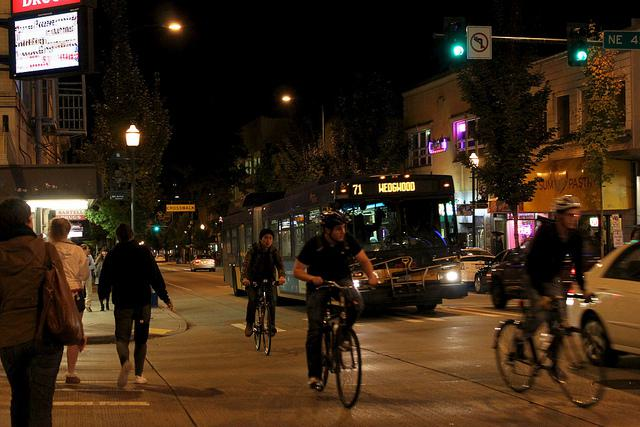
\includegraphics[width=0.4\textwidth]{exp_raw.jpg}}
    \subfigure[SAM-YOLO]{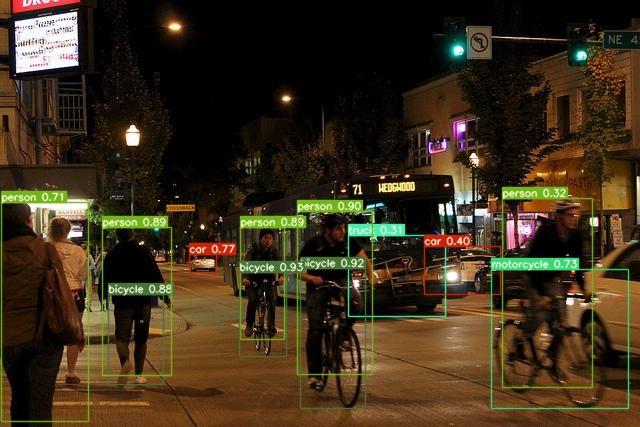
\includegraphics[width=0.4\textwidth]{exp.jpg}}
    % }
\end{figure}

This section analyzes the target detection results on the ExDark dataset \cite{Exdark}, which is designed to evaluate the performance of target detection algorithms under extreme lighting conditions. The analysis covers several algorithms including YOLOv7, SAM-YOLO, CBAM-YOLO, CA-YOLO, SEAM-YOLO, SSD, RetinaNet, and Faster-RCNN. By comparing the performance of each algorithm under two main metrics, $mAP_{0.5}$ and $mAP_{0.5:0.95}$, we aim to reveal the ability of different algorithms to adapt to extreme light change conditions.


In the $mAP_{0.5}$ metric, SAM-YOLO leads the other algorithms with a score of 0.593, which shows that it is more capable of detecting multiple types of objects in the ExDark dataset. Especially in the detection of "bicycle", "tricycle" and "truck", SAM-YOLO shows high accuracy. YOLOv7 also performs well, especially in the "car" category where it achieves a high score of 0.797. In contrast, CBAM-YOLO, CA-YOLO, and SEAM-YOLO perform slightly less well overall, with SEAM-YOLO in particular showing the weakest performance of all categories, probably due to its lack of adaptability to extreme light changes.


On the more stringent $mAP_{0.5:0.95}$ metric, SAM-YOLO leads again with a result of 0.382, further proving its better robustness and accuracy in dealing with complex lighting conditions. In addition, SAM-YOLO performs particularly well in the categories of "tricycle", "car" and "truck", which demonstrates its strong detection ability for large objects. This demonstrates its ability to detect large objects. In contrast, other algorithms such as CBAM-YOLO, CA-YOLO, and SEAM-YOLO perform poorly, especially CA-YOLO and SEAM-YOLO perform lower than expected on most of the categories, which may reflect their shortcomings in dealing with the capture of details under extreme lighting conditions.


By analyzing the test results on the ExDark dataset, we can conclude that the SAM-YOLO algorithm not only performs well under regular lighting conditions but also maintains a high detection performance under extreme lighting conditions. This ability makes it the preferred algorithm for high-precision target detection in complex lighting environments. However, the performance degradation of other algorithms under extreme lighting conditions suggests that improving the robustness of the algorithm to changes in lighting remains an important direction for future research.


\begin{table*}[!htbp]
    \centering
    \caption{Comparison of detection results on ExDark Dataset $mAP_{0.5}$}
    \label{tab:comparative_experiment_ap_5_ExDark}
    \begin{tabular}{ccccccccc}
        \toprule  
 Algorithm   & all   & person & bicycle & tricycle & car   & motorcycle & bus   & truck \\ \midrule
 YOLOv7      & 0.521 & 0.318  & 0.415   & 0.455    & 0.797 & 0.342      & 0.622 & 0.701 \\
 SAM-YOLO    & 0.593 & 0.348  & 0.551   & 0.586    & 0.781 & 0.478      & 0.634 & 0.778 \\
 CBAM-YOLO   & 0.443 & 0.260  & 0.325   & 0.346    & 0.759 & 0.209      & 0.563 & 0.643 \\
 CA-YOLO     & 0.478 & 0.241  & 0.356   & 0.537    & 0.656 & 0.353      & 0.605 & 0.597 \\
 SEAM-YOLO   & 0.309 & 0.152  & 0.138   & 0.129    & 0.694 & 0.127      & 0.454 & 0.468 \\
 SSD         & 0.315 & 0.178  & 0.165   & 0.075    & 0.712 & 0.173      & 0.451 & 0.453 \\
 RetinaNet   & 0.314 & 0.118  & 0.159   & 0.310    & 0.545 & 0.136      & 0.456 & 0.471 \\ 
 Faster-RCNN & 0.310 & 0.139  & 0.238   & 0.196    & 0.543 & 0.141      & 0.401 & 0.508 \\ 
        \bottomrule
    \end{tabular}
\end{table*}

\begin{table*}[!htbp]
    \centering        
    \caption{Comparison of detection results on ExDark Dataset $mAP_{0.5:0.95}$}
    \label{tab:comparative_experiment_ap_95_ExDark}
    \begin{tabular}{ccccccccc}
        \toprule  
 Algorithm   & all   & person & bicycle & tricycle & car   & motorcycle & bus   & truck \\ \midrule
 YOLOv7      & 0.282 & 0.111  & 0.153   & 0.231    & 0.522 & 0.119      & 0.428 & 0.408 \\
 SAM-YOLO    & 0.382 & 0.160  & 0.256   & 0.413    & 0.586 & 0.231      & 0.493 & 0.536 \\
 CBAM-YOLO   & 0.227 & 0.083  & 0.104   & 0.150    & 0.468 & 0.062      & 0.354 & 0.370 \\
 CA-YOLO     & 0.159 & 0.054  & 0.046   & 0.025    & 0.425 & 0.044      & 0.270 & 0.237 \\
 SEAM-YOLO   & 0.142 & 0.039  & 0.037   & 0.040    & 0.367 & 0.028      & 0.268 & 0.211 \\
 SSD         & 0.169 & 0.101  & 0.104   & 0.265    & 0.141 & 0.135      & 0.145 & 0.152 \\
 RetinaNet   & 0.136 & 0.101  & 0.090   & 0.170    & 0.010 & 0.100      & 0.124 & 0.104 \\ 
 Faster-RCNN & 0.157 & 0.008  & 0.084   & 0.142    & 0.087 & 0.078      & 0.124 & 0.104 \\ 
        \bottomrule
    \end{tabular}
\end{table*}\section{Conclusion} \label{sec:conclusion}

In this paper, an improved YOLOv7 algorithm that incorporates a SimAM attention mechanism into the Neck network was proposed, replaces the $CIoU$ function of YOLOv7 with the $SIoU$ function, and simplifies the model architecture to accelerate model training and reduce the number of parameters.  This approach enhances the model's generalization ability, improves the learning of spatial features, and enhances computational efficiency. The results reveal that the SAM-YOLO algorithm outperforms other algorithms in terms of comprehensive performance, especially in terms of accuracy and mAP metrics, both in standard test environments and under extreme lighting conditions. This demonstrates the potential of SAM-YOLO in realizing high-speed and high-accuracy target detection, especially for real-world application scenarios with variable lighting conditions.

Regarding model training, the training set comprises real road videos with a fixed perspective effect, and the proportion of vehicles on the road varies.  Consequently, the model training may result in bias.  To mitigate this limitation, future studies should enhance the original dataset to alleviate the impact of issues related to data collection on the performance of the model.  Furthermore, during the data collection process, non-conventional shooting perspectives like reverse and left-right angles should be introduced to enhance the capability of detecting vehicles in various angles and environments.

Additionally, our findings point to a general decrease in the performance of target detection algorithms under extreme lighting conditions, highlighting the importance of improving the robustness of algorithms to lighting changes. While SAM-YOLO performed the best in these tests, the performance degradation of the other algorithms hints at the need for future work, especially in optimizing the algorithms to better adapt to extreme lighting conditions.

\backmatter

\section*{Declarations}

\subsection*{Funding}

This work is supported by the Natural Science Foundation of Hubei Province (No. 2024AFB147), Xiangyang Science \& Technology Plan (High-tech field, No. 2022ABH006596), Innovation and Entrepreneurship Education Special Project (No. CX2023003).

\subsection*{Conflict of interest}

The author(s) declared no potential conflicts of interest concerning the research, authorship, and/or publication of this article.

\subsection*{Data availability}

The data that support the findings of this study are available from the corresponding author upon reasonable request.

\nocite{*}

% if your bibliography is in bibtex format, use those commands:
\bibliographystyle{sn-mathphys-num}           % Style BST file.
\bibliography{bibliography}        % Bibliography file (usually '*.bib')

\end{document}
